\documentclass[conference]{IEEEtran}
\usepackage{cite}
\usepackage{amsmath,amssymb,amsfonts}
\usepackage{algorithmic}
\usepackage{graphicx}
\usepackage{textcomp}
\usepackage{xcolor}
\usepackage{fancyhdr}
\usepackage[hyphens]{url}
\usepackage{wrapfig}
%\usepackage{subfig}

\usepackage{xpatch}
\makeatletter
\patchcmd\@makecaption{\\}{.~}{}{\fail}
\makeatletter

\def\BibTeX{{\rm B\kern-.05em{\sc i\kern-.025em b}\kern-.08em
    T\kern-.1667em\lower.7ex\hbox{E}\kern-.125emX}}

% Ensure letter paper
\pdfpagewidth=8.5in
\pdfpageheight=11in


%%%%%%%%%%%---SETME-----%%%%%%%%%%%%%
\newcommand{\iscasubmissionnumber}{102}
%%%%%%%%%%%%%%%%%%%%%%%%%%%%%%%%%%%%

\fancypagestyle{firstpage}{
  \fancyhf{}
\renewcommand{\headrulewidth}{0pt}
  \fancyhead[C]{\normalsize{ISCA 2020 Submission
      \textbf{\#\iscasubmissionnumber} \\ Confidential Draft: DO NOT DISTRIBUTE}} 
  \fancyfoot[C]{\thepage}
}  


\pagenumbering{arabic}

%%%%%%%%%%%---SETME-----%%%%%%%%%%%%%
\usepackage{comment}
\newcommand{\red}[1]{\textcolor{red}{#1}}
\newcommand{\blue}[1]{\textcolor{blue}{#1}}
\usepackage{xspace}
\usepackage{listings}
% \usepackage{ulem}
\usepackage{tcolorbox}

\newcommand{\projectname}{RCC\xspace}
%\newcommand{\nowait}{\textsf{\textbf{NOWAIT}}\xspace}
\newcommand{\nowait}{\textsf{\small{NOWAIT}}\xspace}
\newcommand{\waitdie}{\textsf{\small{WAITDIE}}\xspace}
\newcommand{\occ}{\textsf{\small{OCC}}\xspace}
\newcommand{\mvcc}{\textsf{\small{MVCC}}\xspace}
\newcommand{\sundial}{\textsf{\small{SUNDIAL}}\xspace}
\newcommand{\calvin}{\textsf{\small{CALVIN}}\xspace}
\def\step{step } % used for defining every step in cc_algs, can change
\def\system{RCC} % used for defining the name of our framework.

\title{\vspace{-4mm} Comprehensive Evaluation of RDMA-enabled Concurrency Control Protocols \vspace{-15mm}}
\author{}
%%%%%%%%%%%%%%%%%%%%%%%%%%%%%%%%%%%%

\begin{document}
\maketitle
\thispagestyle{firstpage}
\pagestyle{plain}



%%%%%% -- PAPER CONTENT STARTS-- %%%%%%%%
\begin{abstract}

On-line transaction processing (OLTP) applications
require efficient distributed transaction 
execution. When a transaction accesses 
multiple records in remote machines, 
network performance is a crucial factor 
affecting transaction latency and throughput.
Due to its high bandwidth and very low
latency, RDMA (Remote Direct Memory Access) has achieved much higher performance 
for distributed transactions than traditional TCP-based systems. 
RDMA provides primitives for 
both two-sided and one-sided communication.
Although recent works have intensively studied
the benefits of RDMA in
distributed transaction systems,
they either focus on
primitive-level comparison of two 
communication models (one-sided vs. two-sided) or 
only study one concurrency control protocol.
Comprehensive understanding of the implication
of RDMA for various concurrency control protocols
is an open problem. 

In this paper, we build {\em \projectname}, the first
unified and comprehensive RDMA-enabled distributed transaction processing framework supporting 
six concurrency control protocols 
using either two-sided or one-sided primitives.
We intensively optimize the performance
of each protocol without bias,
using known techniques such as co-routines, outstanding requests, and
doorbell batching.
Based on \projectname, we conduct the first
and most comprehensive
(to the best of our knowledge) study
of the six representative distributed
concurrency control protocols 
on two clusters with different 
RDMA network capabilities.





%Distributed database management systems (DBMS) have long been using concurrency control protocols like 2-phase locking (2PL)~\cite{Bernstein:1981:CCD:356842.356846}, multi-version CC (MVCC)~\cite{bernstein1983multiversion} and Optimistic Concurrency Control (OCC)~\cite{kung1981optimistic} to ensure atomicity and serializability of distributed transactions. Other concurrency control protocols like CALVIN\cite{Thomson:2012:CFD:2213836.2213838}, 
% MaaT~\cite{mahmoud2014maat} 
%and Sundial~\cite{yu2018sundial} have also been proposed in recent years. Meanwhile, High-speed network technology like Remote Direct Memory Access (RDMA) is getting popular and used by recent transaction processing systems like DrTM~\cite{wei2015fast} and RTX~\cite{wei2018deconstructing} due to its low latency. Unfortunately, it is hard to compare and evaluate concurrency control protocols under the context of using RDMA. We developed RCC, a framework containing various representative build-in concurrency control protocols with RDMA support. we provide detailed designs and evaluations of each protocol in terms of both using RDMA-enabled RPC and using one-sided RDMA primitives. As far as we know, this is the first framework where researchers can compare different concurrency control protocols on one single system under the context of RDMA.

\end{abstract}

%\vspace{-2mm}
\section{Introduction}
%\vspace{-1mm}
%\vspace{-1mm}
%-- The importance and challenges of distributed 
% transactions. (from VLDB 1st and 2nd paragraph of introduction)

On-line transaction
processing (OLTP) has ubiquitous 
applications in important domains including
banking, stock marketing, e-commerce, etc. 
As the exponential growth of data volume, single-server Database Management Systems (DBMS) are experiencing extreme difficulties to handle a large number of queries from clients due to limited system resources. Partitioning data sets across distributed machines is
necessary and becoming increasingly important. 
%becoming increasingly necessary and important. 
However, it has been shown that partitioning data such that all queries access only one partition is challenging~\cite{curino2010schism,pavlo2012skew}. Therefore, it is unavoidable to execute distributed transactions that access 
a set of networked machines. 

Distributed transactions should guarantee:
(1) atomicity: either all or none of the machines agree to apply the updates; and
(2) serializability: all transactions must commit in some serializable order. 
%must have the following properties 1) atomicity. Either all machines agrees to apply the changes or none of them does. 2) serializability. All transactions must commit changes as if they commit in some serializable order. 
To ensure these properties, distributed transactions have been intensively for decades.
%there has been a large amount of studies in the database community about distributed transactions since the 1980's. 
Prior works have proposed many distributed concurrency control protocols such as 2-Phase Locking (2PL)~\cite{Bernstein:1981:CCD:356842.356846}, timestamp-based~\cite{Bernstein:1981:CCD:356842.356846}, multi-versioned~\cite{bernstein1983multiversion}, optimistic concurrency control (OCC)~\cite{kung1981optimistic}, etc. % MaaT~\cite{mahmoud2014maat}etc. 

The well-known challenge of multi-partition serializable concurrency control protocols
is the significant performance 
penalties\cite{stonebraker1986case}~\cite{Thomson:2012:CFD:2213836.2213838}.
When a transaction accesses multiple records over the network, any other transactions it conflicts with have to be serialized~\cite{bailis2014coordination}. Therefore, a high-speed network plays a crucial role in a distributed DBMS system.


% -- Performance advantage of RDMA and fast network. (1st paragraph of OSDI in introduction) 

Remote Direct Memory Access (RDMA) is a
new technology that enables the network interface card (NIC) to access the memory of a 
remote server in a distributed cluster. 
Due to its high bandwidth and very low
latency, RDMA has been actively used in distributed transaction systems~\cite{wei2015fast,kalia2016fasst,chen2016fast,dragojevic2015no} and has enhanced the performance by orders of magnitude compared to traditional systems using TCP/IP. 

RDMA network supports both TCP-like 
{\em two-sided} communication using primitives \texttt{SEND/RECV}, and
{\em one-sided} communication using 
primitives \texttt{READ/WRITE/ATOMIC},
which are capable of accessing remote memory while bypassing traditional network stack,
the kernel, and even remote CPUs. 
To understand the performance of these primitives, there has already been 
intensive studies investigating the 
pros and cons of using each primitive. 
Recently, several works compared two-sided primitives versus one-sided ones~\cite{kalia2014using,dragojevic2014farm,dragojevic2015no,wei2018deconstructing,tsai2017lite} at  {\em primitive-level} using micro-benchmarks. 



Unfortunately, primitive-level comparisons do not directly transfer to insights of
building high-performance transaction processing systems. 
How to effectively leverage the two types of primitives is still a difficult consideration. 
Two takeaways from recent work RTX~\cite{wei2018deconstructing} are: 
(1) the best performance of a specific concurrency control protocol (i.e., OCC) cannot be simply achieved by solely using one-sided or two-sided communication; and 
(2) different communication primitives 
are suitable for different protocol {\em stages}. 
These conclusions suggest 
that achieving the best performance of a concurrency control protocol using RDMA technology is far from trivial and demands a systematic investigation. 

Recent works such as \cite{kalia2016fasst,dragojevic2014farm,wei2018deconstructing} all focus on the design and optimization of \occ using RDMA. 
However, with a great number of other well-known
and important concurrency control protocols~\cite{mu2014extracting,mahmoud2014maat,roy2015homeostasis,escriva2015warp,cowling2012granola}, 
the best implementation practices using 
RDMA and its implication 
on {\em different protocols} are still unknown. 
Specifically, we ask several key
{\bf open questions}: 
(1) For each protocol, {\em how} to leverage 
RDMA to construct an efficient implementation?
(2) For each protocol, between two-sided 
and one-sided communication, {\em which} choice
can achieve better performance?
(3) In the context of RDMA, how can we perform
{\em apple-to-apple} comparison among the 
performance and characteristics of 
{\em different} protocols?
(4) For different protocols, what are the 
implications of RDMA network performance? 
Are the implications similar or largely different?
What is the relative performance of different
protocols with RDMA compared to TCP~\cite{harding2017evaluation}?
The list of questions can go on and on. 
Unfortunately, current research on RDMA-enabled distributed transaction systems is insufficient
to answer these critical questions. 

%What would a detailed one-sided implementation be like for a protocol If there hasn't been one? 

%(2) Which is a better way to implement a protocol, two-sided-primitive based remote procedure call (RPC) or one-sided primitives? 

%(3) Can we perform an fair and apple-to-apple
%comparison among all these RDMA-based protocol implementations in a unified framework? 

%(4) what's the implication of RDMA network performance on protocols' behavior? All these questions are open problems 
%unanswered in the existing work.

In this paper, we take the first step to
provide definitive answers to the above questions. 
We build {\em \projectname}, the first
unified and comprehensive RDMA-enabled distributed transaction processing framework supporting 
{\em six} concurrency control protocols including
\nowait~\cite{Bernstein:1981:CCD:356842.356846}, \waitdie~\cite{Bernstein:1981:CCD:356842.356846}, \occ~\cite{kung1981optimistic}, \mvcc~\cite{bernstein1983multiversion}, \sundial~\cite{yu2018sundial}, and 
\calvin~\cite{Thomson:2012:CFD:2213836.2213838}.
Based on \projectname, we conduct the {\em first
and most comprehensive} 
(to the best of our knowledge) comparison
of {\em different} representative distributed
concurrency control protocols in the context 
of RDMA. 
%We attempt to answer these questions by building \textbf{\system} -
%the first unified RDMA-based transaction processing framework for evaluating representative distributed 
%concurrency control protocols. 
The wide range of protocols supported in \projectname includes: (1) classical protocols
that have been used in production DBMS
for decades such as 2PL (\nowait and \waitdie);
(2) \occ, which has attracted most recent research 
interests; (3) \mvcc and \sundial,
which use timestamp to allow more concurrency;
and (4) \calvin, a recently proposed protocol
to ensure deterministic transaction execution.
We believe that the diverse set of protocols
can well represent recent 
research trends and industry
practices of concurrency control algorithms.
It is imperative to understand
the potential and implication of RDMA technology
in this context. 

%We consider classic protocols that have been used in real DBMS industry for decades like 2-phase locking with both no-wait and wait-die deadlock prevention strategies as well as timestamp-based multi-version protocol. Meanwhile, we consider  recently proposed protocols like CALVIN\cite{} and Sundial\cite{}. CALVIN is a deterministic protocol. Sundial is the state-of-the-art protocol which is capable of integrating with cache coherence. They represent recent trends on the development of concurrency control protocols thus worth our attention. 

In \projectname, we provide two implementations
for each protocol: using {\em two-sided} 
RDMA-enabled Remote Procedure Call (RPC)
and one-sided communication primitives.
We intensively optimize the performance
without bias
using known techniques such as co-routines~\cite{kalia2016fasst}, outstanding requests~\cite{wei2018deconstructing},
doorbell batching~\cite{kalia2016design}.
We evaluated all protocols in \projectname
on {\em two clusters} with different 
RDMA network capabilities.
One is equipped with ConnectX-4 EDR 100Gb/s InfiniBand (EDR) and the other with ConnectX-3 Pro FDR 56Gb/s InfiniBand (FDR).
We use them due to the huge difference in supporting RDMA one-sided operations: the latency of a single one-sided operation using FDR InfiniBand can be 5x more than that of using the EDR InfiniBand. We evaluate \projectname on three OLTP workloads: 
SmallBank~\cite{SmallBank}, TPC-C~\cite{TPC-C}, and
YCSB~\cite{cooper2010benchmarking}. 

Compared to RTX~\cite{wei2018deconstructing} which only studied \occ, \projectname covers
significantly more representative protocols,
providing the opportunity to perform
a much more comprehensive study and revealing 
more insights. 
%opening up new possibilities for us to conduct a more extensive study on the impact of using RDMA on different concurrency control protocols and compare these protocol under the context of RDMA. 
Compared to Deneva~\cite{harding2017evaluation}, the latest in-memory distributed database evaluation framework also including six 
(slightly different) concurrency control protocols, \projectname
implements each protocol using
RDMA communication primitives 
instead of TCP/IP, providing more guidelines and insights for building RDMA-friendly protocols.

%Based on \projectname, we have the following 
%findings:
%\red{SUMMARIZE THE FINDINGS HERE}

\begin{comment}
\begin{itemize}
    \item For workloads with more computation (CPU bound), one-sided is better since it bypasses the remote CPU. Its advantage grows with increasing computation workloads.
    \item 
    %We can different conclusion for ONESIDED and RPC version to choose protocols. 
   % For one-sided, we should trade off between the simplicity and the flexibility of the protocols considering the conflict rate. 
   More advanced protocols reduce abort rate while launching more RDMA one-sided operations. 
   For RPC, they are better in all condition because the protocols will only increase the number of local operations while reducing the abort rate.
    \item For workloads with less computation and low contention, one-sided \occ is the best
    due to its simple and low number
    of network operations.
    For workloads with higher contention, protocols like one-sided \mvcc and \sundial are better choices because they have optimization to reduce read-write conflict.
    %and nearly the same cost with other protocols when abort.
    %\red{With higher contention, ...}
    \item For workloads bounded by network with low contention, increasing the number of
    co-routines leads to higher throughput.
    \item Even if ConnectX-3 has poor support for RDMA one-sided operations, increasing the number of co-routines is still beneficial 
    when transactions have more computation.
\end{itemize}
\end{comment}





%For each selected protocol in \system, we implemented both two-sided RPC version and one-sided version and leveraged existing optimization techniques like co-routines and door-bell batching to intensively optimize the performance. We evaluated all protocols in \system\ on two clusters with different RDMA network capabilities against three  OLTP (Online Transaction Processing) workloads: banking, TPC-C, YCSB and identified a preferable method of communication.


% several recently 
% proposed protocols.... similar to VLDB. 
% We leveraged the existing optimization techniques
% such as ... (co-routine, door bell, etc.) to 
% intensively optimize the performance of each
% protocol. 
% We identified the best option (RPC vs. RDMA) for different phases in each protocol and provide two
% implementations: RPC-only and mostly RDMA with 
% some operations in RPC. 

% performance of OCC. 
% Different protocols have different phases,

% how to achieve the best performance is far from trivial. OSDI shows the design and optimization
% for OCC, but not other protocols. Thus, 
% the suitability of RDMA on the existing concurrency
% control protocols and the best design and optimization for each are unknown. 

% -- We ask the following 
% questions: 
% (1) what's the best way to implement
% each protocol, RPC or RDMA or hybrid? What are the detailed implementations? (OSDI only
% answers it for OCC).
% (2) can we perform the fair and apple-to-apple
% comparison of the protocol implementations with 
% RDMA in a unified framework? (VLDB only compares
% the implementations based on RPC and stored procedure).
% (3) what's the implication of RDMA network performance on protocols' behavior? (OSDI only 
% shows results based on one RDMA setting)
% All these questions are open problems 
% unanswered in the existing work.

% -- We attempt to answer these questions by building
% the first unified RDMA-based framework for distributed 
% transactions. We consider several recently 
% proposed protocols.... similar to VLDB. 
% We leveraged the existing optimization techniques
% such as ... (co-routine, door bell, etc.) to 
% intensively optimize the performance of each
% protocol. 
% We identified the best option (RPC vs. RDMA) for different phases in each protocol and provide two
% implementations: RPC-only and mostly RDMA with 
% some operations in RPC. 

% -- Emphasize it is the first such framework. 
% Compared to OSDI, ...
% Compared to VLDB, ...
% In the evaluation, we use **two** clusters
% with different RDMA network performance and 
% XXX applications to 
% investigate the implications for RDMA-based
% implementations and different protocols. 
% It is also the first paper that perform such 
% study on two cluster. 

%-- Summarize our key findings. 
%(1) RPC vs. RDMA (mostly), which one is better? In which condition? (With high network performance, RDMA is better? Otherwise, RPC?)
%(2) Not all phases are suitable for RDMA? For example, .. mention all findings. 
%(3) Which optimizations are important?
%(4) .... (write more based on the results).

%To conclude, for applications with little execution workload(small bank), RPC is the better choice for 

%-- Paper structure.




%\vspace{-2mm}
\section{Background}
%

%\vspace{-2mm}
\subsection{RDMA and Its Primitives}
%\vspace{-2mm}

%-- Similar to OSDI's corresponding section. 

RDMA (Remote Direct Memory Access) is a network technology featuring high bandwidth and 
low latency data transfer with low CPU overhead. 
%transfer data in  low latency and high bandwidth while incurring low CPU overhead. 
It is widely considered suitable for large data centers. RDMA operations, a.k.a, \textbf{verbs}, can be classified into two types:
(1) {\em two-sided} operations including RDMA
\texttt{SEND/RECV}; and 
(2) {\em one-sided} operations including RDMA
\texttt{READ/WRITE/ATOMIC}.
The latter provides the unique capability to directly access the memory of remote machines without involving remote CPU. 
This feature makes one-sided operations suitable for distributed applications with high CPU utilization. 
Although having similar semantics with TCP's send/receive over bound sockets,
%These are the build in .. for tpc (\blue{TODO: there is a sentence in another section which describe the relationship between tcp and two-sided well, i didn't find it}). 
RDMA two-sided operations bypass the tranditional network stack and the OS kernel, 
making the performance of 
RPC implementation over RDMA much higher than
that over TCP/IP.


%The first type is one-sided operations including RDMA READ, RDMA WRITE and RDMA ATOMIC. One-sided operations are special in RDMA since they can directly access the memory of a remote machine without involving the remote CPU. This feature makes one-sided operations suitable for distributed applications with high CPU utilization. 
%The other type is two-sided RDMA operations, including RDMA SEND and RDMA RECV. Although having similar semantics with TCP's send/receive over bound sockets,
%These are the build in .. for tpc (\blue{TODO: there is a sentence in another section which describe the relationship between tcp and two-sided well, i didn't find it}). 
%they bypass the tranditional network stack and the OS kernel, making the RPC implementation over RDMA outperform that over TCP/IP.

Queue pairs (QPs) must be set up for RDMA communication. A QP consists of a send queue and a receive queue. When a sender posts an one-sided RDMA request to the send queue, the local QP will transfer data to some remote QP, and the sender can poll for completion information from the completion queue associated with the QP.
%once the operation is completed. 
The receiver's CPU is not aware of the one-sided operations performed by receiver's RNIC without checking the changes in memory. For a sender to post a two-sided operation, the receiver QP has to post RDMA \texttt{RECV} for the corresponding RDMA \texttt{SEND} in advance. It polls the request from the receive queue to obtain the incoming data.

QP has three different transport modes: Reliable Connection (RC), Unreliable Connection (UC) and Unreliable Datagram (UD). One RC QP can send messages reliably to exactly one another connected RC QP; a UD QP can either uni-cast to one or multi-cast to many UD QPs without delivery guarantee. One-sided operations are only fully supported between two RC QPs, while two-sided operations must be used for UD QPs. To set up a reliable connection, a node has to maintain a cluster-size number of QPs in its RDMA-enabled NIC (RNIC) at least, each connected with one remote node. On contrary, a node just needs to maintain one UD QP to send/receive data across the cluster, thus saving system resources.

%\vspace{-2mm}
\subsection{RDMA-enabled Distributed Transactions}
%\vspace{-2mm}
%-- Similar to OSDI's corresponding section. 

Distributed transaction systems are popular applications with demanding network operations. 
Intensive research has been conducted
on using RDMA to support distributed transactions. \cite{chen2016fast} uses pure one-sided operations to transfer and update records. \cite{kalia2016fasst} uses UD to implement RPC in its transaction framework. \cite{wei2018deconstructing} brings up a hybrid of one-sided and two-sided operations for different stages of transactions. All these frameworks focus on some variant of \occ~\cite{kung1981optimistic}.

%\blue{osdi here follows the introduction for occ, we do not need it}

%\subsection{Concurrency Control Protocols}

%-- Summarize the protocols we implemented in this paper. No need to discuss implementation details, but use 1-2 sentences for each to provide the insights
%and main goal for each protocol. 

\begin{comment}
As transactions are executed concurrently,
concurrency control algorithms are designed 
to guarantee the correct semantics, e.g. atomicity and serializability. 
Two main design goals of various algorithms 
are reducing abort and increasing throughput.
As examples of 2PL algorithms,
\nowait and \waitdie both resolve conflicts 
by aborting one of transactions, also 
avoiding deadlock. 
\waitdie assigns priority to transactions
and makes abort decisions based on it to 
avoid unnecessary aborts. 
%When acquiring the locks, NOWAIT will abort immediately when finding a record already locked. While WAITDIE has a global consensus about the priority. The one with higher priority will keep waiting for the lock to be released and the one with lower priority will abort at once. This avoids some unnecessary aborts. 
Different from 2PL, \occ reads data without locking and optimistically assumes 
that the conflicts between transactions are low.
It performs validation before commit. 

%\occ first reads data without locking,
%after execution with the data, 
%it will validate the data by reading write lock, and commit transaction 
%write time stamp and write back the updated data after acquiring the lock. If therr is low contention, OCC works very well. But it will be rather worse if the contention is high because it can only validate the data after execution, which leads to high abort cost. 
\sundial is a combination of 2PL and OCC algorithm. It does not use read lock. Instead, it preserves the read lease and dynamically changes it. It validates the reads based on write time stamp. However, by preserving the read lease and locking the writes, it can validate the transaction before the execution, which makes the abort in Sundial less costly.

\end{comment}



\section{System Overview}
%\vspace{-2mm}
%-- Similar to Section 2 of VLDB, need a figure similar to Figure 1 of that paper

% \vspace{-2mm}
\subsection{Principles and Architecture}
%\vspace{-2mm}


%-- Based on the figure, explain the overall design flow shared by all protocols. I understand that the design is based on ROCC, so the figure will be  different from VLDB. You need to draw a figure based on ROCC framework and describe the common interface and components for all protocols. 

%In order to implement and evaluate representative concurrency control protocols using RDMA primitives, we designed a framework called \textbf{\system}. 
\setlength{\intextsep}{2pt}%
\setlength{\columnsep}{8pt}%
\begin{wrapfigure}[10]{r}{0.60\linewidth}
%\begin{figure}[t]
    \centering
    \vspace{-0.2cm}
    \includegraphics[width=\linewidth]{images/System.pdf}
    \vspace{-6mm}
    \caption{RCC Framework Overview}
    \vspace{-0.8cm}
    \label{fig:system}
\end{wrapfigure}
Figure~\ref{fig:system} shows the overview of 
\projectname, which runs on multiple symmetric distributed nodes,
each contains a configurable number of server threads 
to process transactions. A client thread continuously sends transaction requests to a random transaction processing thread in the cluster. The stats thread is used to collect the statistics (e.g., the number of committed transaction) generated by each processing thread. The QP thread is used to bootstrap RDMA connection by establishing the pairing of RDMA QPs using TCP connections. 

\projectname uses co-routines as an key optimization technique~\cite{kalia2016fasst} for hiding network latency. To this end, each thread starts an {\em event handling} co-routine and a number of {\em transaction coordination} co-routines. An event handling co-routine continuously checks and handles network-triggered events such as polled completions or {memory-triggered events} such as the releasing of a local lock. A transaction coordination co-routine is where a transaction is logically executed.

In \projectname, the distributed in-memory database is implemented as a distributed key-value store which can be accessed either locally or remotely via a key and table ID. In addition to the in-memory database, each protocol has its protocol-specific metadata to serialize transaction execution. For some protocol like \calvin, protocol-specific RDMA buffers are required for collecting transaction inputs and forwarding local reads. 

%\vspace{-2mm}
\subsection{Transaction and Execution Model}
%\vspace{-2mm}

%-- See VLDB paper, but our model is **not** based on stored procedure. Explain our model here: how data are distributed? server/client. (Also check OSDI paper, it also mentioned ``symmetric model''..)
\projectname employs a symmetric model to execute transactions: each node serves as both a client and a transaction processing server. As shown in Figure~\ref{fig:system}, each transaction coordination co-routine is responsible for executing a transaction at any time. 
We use {\em coordinator} to refer to the co-routine which receives transaction requests from some local or remote client thread and orchestrates transactional activities in the cluster. We use {\em participant} to refer to a machine where there is a record to be accessed by some transaction. When a 
participant receives a RPC request, its event handling co-routine will be invoked to process the request locally.
When a participant receives a RDMA one-sided 
operation, its RNIC is responsible for accessing the memory without interrupting the CPU.

In \projectname, the in-memory database keeps all records. Since one-sided operations can only access remote memory by leveraging the pre-computed remote offsets. To reduce the number of one-sided operations involved in retrieving metadata, they are placed physically together with the record
as shown in Figure~\ref{fig:metadata}.
A {\em record} refers to the 
actual data and a {\em tuple} refers to record associated 
with the relevant metadata.


A transaction contains reads and writes of 
records that are performed atomically.
The execution of a transaction contains three
stages~\footnote{We use this assumption for simplicity. The implementation
can also be applied to transactions with multiple fetching and execution stages.}: 
1) {\em fetching}, in which a read/write operation fetches the record and/or metadata if needed;
2) {\em execution}, in which a transaction  performs the actual computation locally using the record just fetched; and 
3) {\em commit}, in which a transaction checks the metadata to find out if the transaction execution is serializable. 




\begin{comment}
In our \projectname, 
%we assume that each transaction will only have one commit stage, which means the transaction will end after committing. To make our introduction more concise, 
we assume that there is just one data fetching and execution stage. However the implementation
can be applied to transactions with multiple date fetching and execution stages.
The execution of each read and write is
composed of three stages:
1) {\em access} the data and add the operation into {\em read or write set};
2) {\em validate} the operation; and 
3) {\em commit} the write set when the transaction

Generally, a transaction execution is divided into three stages, and consists of write or read operations. The first stage is \textbf{fetching}, where the write or read operation  fetches the needed record. The second stage is \textbf{execution}, where the transaction will do the actual computation locally using the record just fetched. The third stage is \textbf{commit}. In this stage, the transaction checks the metadata to find out if the execution was valid. after which it commits the updated records as well as their corresponding metadata.
\end{comment}

%\vspace{-2mm}
\subsection{RDMA Primitives and Optimizations}
%\vspace{-2mm}

% -- See 3.1 and 3.2 of OSDI, try to be brief since they are not our contribution. Also mention any optimizations we have proposed and validated to work well. 



We uses two-sided RDMA primitives (i.e., \texttt{SEND/RECV}) over UD QP in the
implementation of RPC. From ~\cite{kalia2016fasst},
two-sided primitives over UD QPs have better performance for symmetric transaction systems \red{than one-sided} and UD mode is much more reliable than expected with RDMA network's lossless link layer. \cite{wei2018deconstructing} further confirms the unsuitability of one-sided primitives to implement fast RPC compared to two-sided ones. 


Figure~\ref{fig:two-vs-one-primitives} illustrates the two types of communications in \projectname by each concurrency control protocol. In two-sided RPC, a coordinator first sends a memory-mapped IO (MMIO) to the RNIC, which will \texttt{SEND} a RPC request to the receiver's RNIC. After the corresponding participant \texttt{RECV}s the request, its CPU will poll a completion event, 
which will trigger a pre-registered handler function to process the request and send back a reply using similar verbs. In one-sided communication, after the participant receives a one-sided op request (i.e., \texttt{READ}, \texttt{WRITE}, \texttt{ATOMIC}), its RNIC will access local memory using a Direct Memory Access (DMA). The completion is signaled when the coordinator polls if it is interested in the completion event.

\setlength{\intextsep}{2pt}%
\setlength{\columnsep}{8pt}%
\begin{wrapfigure}[8]{r}{.55\linewidth}
%\begin{figure}[htp]
    \centering
    \vspace{-0.2cm}
    \includegraphics[width=\linewidth]{images/two_vs_one.pdf}
    \vspace{-1cm}
    \caption{Two-sided v.s. one-sided primitives}
    \vspace{-0.4cm}
    \label{fig:two-vs-one-primitives}
\end{wrapfigure}
MMIO is an expensive operation to notify RNIC of a request fetching event. Therefore using one MMIO for a batch of RDMA requests can effectively save PCIe bandwidth and improve the performance of transaction systems~\cite{wei2018deconstructing}. Meanwhile, having multiple outstanding  requests on the fly can help save the waiting time of request completions, thus reducing the latency of remote transaction~\cite{wei2018deconstructing}. Besides co-routines, \projectname uses similar techniques as important optimizations.

\section{Concurrency Control Protocols}
%\vspace{-2mm}

%-- Describe each protocol design in detail, explain the ideas well. If you made some design choices based some considerations or tradeoffs, please also put them here. 

%-- Do not mention OCC as the baseline, just discuss
%all protocols in some order. When talking about OCC, mention that it is based on the OSDI (with any modifications). 

%-- For each protocol, remember to describe both: RPC and (mostly) RDMA. Draw some figures if needed, especially for the protocols that incurred significant coding/debugging (e.g. Calvin). 

%-- I remember that you mention certain operations are needed by all (or several) protocols and it is best to use RPC/RDMA to implement them. Please discuss them in the final "Discussion" section, and perhaps add a table with {operations, protocols} indicating any design options and findings in each cell. 

In \projectname, we implement six concurrency control protocols 
with RDMA-enabled
two-sided and one-sided communication primitives. 
The implementations of these protocols
involve a variety of techniques. 
%The concurrency control algorithms that we primarily concern and included in our system cover a diversity of different techniques. 
%These protocols can be classified into several types. 
Among these protocols,
\nowait~\cite{Bernstein:1981:CCD:356842.356846} and \waitdie~\cite{Bernstein:1981:CCD:356842.356846} are two examples of 2-phase locking (2PL)~\cite{Bernstein:1981:CCD:356842.356846} 
concurrency control algorithm.
They differ in conflict resolution --- how conflicts are handled to ensure serialization. 
%We will have a detailed discussion in their respective subsections. 
Compared to 2PL, Optimistic Concurrency Control (\occ)~\cite{kung1981optimistic} reads records speculatively without locking and 
validates data upon transaction commits 
--- the only time to use locks. 
%OCC constraints locking only to the time when transactions commit. 
\mvcc~\cite{bernstein1983multiversion} optimizes the performance of read-heavy transactions by allowing the read of stale records instead of aborting. \sundial~\cite{yu2018sundial} leverages dynamically changing logical leases to determine the transaction commit orders and reduce aborts. 
\calvin~\cite{Thomson:2012:CFD:2213836.2213838} introduces determinism to sequence transaction inputs and schedule transactions in a deterministic fashion. 

\begin{figure}[t]
    \centering
    \vspace{-1mm}
    \includegraphics[width=8cm]{images/CC-data.pdf}
    \vspace{-5mm}
    \caption{Metadata for Concurrency Control protocols}
    \vspace{-8mm}
    \label{fig:metadata}
\end{figure}

While the protocols themselves are known before, 
the new contribution of 
\projectname is to rethink their {\em implementation in the context of RDMA}. 
For each protocol, we implement two versions:
1) RPC version, which mostly uses remote function call enabled by RDMA's two-sided communication primitives (i.e., \texttt{SEND/RECV}); 
and 2) one-sided version, which mostly uses RDMA's unique 
one-sided communication primitives (i.e., \texttt{WRITE/READ/ATOMIC}). 
Each version does not solely use
one type (one- vs. two-sided) of RDMA primitives
--- we choose the proper primitives
to implement certain operations when the alternative
is overwhelmingly worse. 
%Next, we first discuss the common
%transaction structure and operations. 

%Currently, there are two major means of inter-nodes communication using RDMA. 1) Remote Procedure Call (RPC) using two-sided RDMA primitives (i.e.,  SEND/RECV). This is a natural drop-in replacement of RPC using TCP. 2) One-sided primitives such as WRITE/READ/ATOMIC operations. Figure~\ref{fig:two-vs-one-primitives} illustrates these two different types of communications.

%\vspace{-2mm}
\subsection{Design Principle}
%\vspace{-2mm}
% TODO: the name of stages in one operation and in one transaction
 
%is committed.
%In the implementation of each protocol by RDMA
%primitives, we should consider the trade-offs
%between one- and two-sided communication. 
The trade-off between two-sided and one-sided 
RDMA primitives is well-known. 
In RPC version, 
operations are sent to and executed on the
remote machine. 
The advantage is that the whole operation can be done with one function call, saving communication.  
But the local machine needs to 
wait for the remote execution which is typically done by
a co-routine after the remote CPU is interrupted.
In contrast, one-sided primitives 
bypass remote CPU and typically achieve
better performance for 
applications with higher CPU usage.
However, it may launch more network 
requests and needs to maintain metadata for remote offsets. 
%whenever remote data is needed. 
%Moreover, metadata need to be maintained to keep
%remote offsets. 
Also, one-sided atomic
operation tends to be costly. 
Based on these trade-offs, we consider several common operations used in concurrency control protocols. 

{\bf Locking.} Locking is needed in all six protocols. The implementation choice depends on the load of remote machines executing co-routines. If it has longer co-routine
execution time, the remote lock handler in RPC version will wait longer, and one-sided implementation is better. 
We observe this behavior in YCSB 
in which the co-routine
execution time can be configured in the benchmark. 
For TPC-C and SmallBank, RPC implementation is better
since the co-routine execution time is short. 

{\bf Validation. } This operation is needed
in \occ, \mvcc, and \sundial.
RPC version just needs one network operation, 
but similar to locking, the best choice also depends on 
the co-routine execution time in remote machines. 

%but the RPC execution time needs to be considered.
%Similar to locking, the best choice is determined 
%by the co-routine execution time in remote machine. 

{\bf Commit. } It is needed in all protocols.
Except for \calvin, which only commits locally, one-sided 
implementation is better since the operation normally just needs to write updated data in a remote machine. Moreover, the overhead of accessing metadata can be avoided by caching them in advance.

Next, we describe the implementation 
of five concurrency control protocols except for \occ, which
is implemented based on RTX~\cite{wei2018deconstructing}.
We try our best to give detailed descriptions so that
the paper can also serve as a reference for others to implement 
the protocols in RDMA. No prior work has shown the comprehensive 
designs and we will also open source our framework if the paper is accepted. 






% As \cite{} suggests, RPC with two-sided RDMA is more appropriate for CScenarios of discrepant needs may benefit from different usage of RDMA. CPU-bound situations, i.e., situations that needs far more local computation than network communications. Otherwise, one-sided primitives are preferred to eliminate the necessity of remote CPU involvement. 

% design overview
% For both RPC and ONEISDED version, we just have to implement three stages of the transaction within three function, that is, read/write, load\_read/load\_write and commit.

%\vspace{-2mm}
\subsection{NOWAIT}
%\vspace{-2mm}


 
\nowait~\cite{Bernstein:1981:CCD:356842.356846} is a basic concurrency control algorithm 
based on 2PL that prevents the deadlocks. 
%is the most basic way of deadlock prevention mechanism among 2-phase locking concurrent control algorithms. 
%It was proposed by ~\cite{Bernstein:1981:CCD:356842.356846} in the 1980s. 
A transaction in \nowait tries to lock all the records accessed, if it fails to lock a record that is already locked by another transaction, 
the former transaction aborts immediately.
%to prevent deadlock. 
Figure~\ref{fig:nowait} shows our RPC and one-sided implementations of \nowait. 

{\bf RPC}
%In the RPC implementation,
%is straight forward. As shown in Figure~\ref{fig:nowait}, 
In data fetch stage, the locking of read/write
 records is done by sending RPC locking request
to the corresponding participant (\step \textbf{a1}).
%will trigger the send of an RPC request for locking
%to the corresponding participant (\step \textbf{a1}).
%sending locking a RPC request to each corresponding participant (\step \textbf{a1}). 
An RPC handler is called to lock the record using local CAS (\step \textbf{a2}). If the CAS fails, a failure message is sent back and the coordinator will release all read and write
locks by posting RPC release requests before aborting the transaction (\step \textbf{a3}).
%\red{WHAT OPERATION DO WE USE FOR 
%RELEASING LOCK? ONE-SIDED?}. 
After successfully locking the record, the coordinator buffers its key and the corresponding participant's ID. The coordinator then sends a read/write 
request to the corresponding participant in another RPC 
using the buffered information (\step \textbf{a4}). By executing the handler, the participant looks for the record locally (\step \textbf{a5}). After all records are collected, the transaction is executed locally at coordinator side.
At commit stage, 
a write back request with the updated record 
is sent back to each participant (\step \textbf{a6}), where an RPC handler 
performs write back of the record and releases the lock (\step \textbf{a7}).

{\bf One-sided }
In data fetch stage, RDMA atomic operations 
\setlength{\intextsep}{2pt}%
\setlength{\columnsep}{8pt}%
\begin{wrapfigure}[10]{r}{.50\linewidth}
%\begin{figure}[htp]
    \centering
    \vspace{-0.4cm}
    \includegraphics[width=\linewidth]{images/NOWAIT.pdf}
    \vspace{-0.8cm}
    \caption{\nowait Implementations}
     \vspace{-0.4cm}
    \label{fig:nowait}
\end{wrapfigure}
are issued by the coordinator to lock remote records (\step \textbf{b1}). The transaction aborts if the RDMA \texttt{CAS} fails (\step \textbf{b2}). In the same \step \textbf{b1}, the coordinator issues an RDMA \texttt{READ} immediately after the RDMA \texttt{CAS} using the offset of remote record to load the record
since the record cannot be changed if the lock succeeds. 
In case of failed locking attempt, the returned record is simply ignored. 
The read offsets are collected and cached by the coordinator before transaction execution starts and thus 
do not incur much overhead.
At commit stage, two RDMA \texttt{WRITEs} are posted to update and unlock the record (\step \textbf{b3}). Only the second RDMA write is signaled to avoid sending multiple MMIOs and wasting PCIe bandwidth. Such doorbell batching mechanism
provides an efficient way to issue multiple outstanding requests from the sender.
This optimization is also used in RTX~\cite{wei2018deconstructing}. 
Based on this, only one yield is needed after the last request is posted, and
we can reduce latency and context switching overhead.

%Since the record of the tuple cannot be changed after being locked, we read the data \emph{right after} locking the tuple by doorbell-batching an RDMA \texttt{CAS} with an RDMA \texttt{READ} in step \textbf{b1}. 
%The \texttt{CAS} might fail when the remote tuple is locked, and then the record retrieved from the second \texttt{READ} is ignored. 
With high contention, lock\&read doorbell batching tends to add 
wasted network traffic. For 
network intensive applications with low contention (i.e., SmallBank), the throughput will increase by 25.1\% while average latency decreased by 22.7\% 
with the above doorbell batching optimization.
The lock\&read in data fetch stage and the update\&unlock in the commit stage with doorbell batching are used in one-sided implementation of five protocols except \calvin. 
%As discussed before, the one-sided version of
%commit operation is more efficient than RPC version.

%\vspace{-2mm}
\subsection{WAITDIE}
%\vspace{-2mm}


%\waitdie is another 2PL algorithm based on a
%different conflict resolution policy. 
It avoids the drawback of \nowait --- unnecessarily aborting any transactions accessing conflicting record.
%as a deadlock prevention technique. 
Instead, it resolves the conflicts with the globally consensus priority, i.e., a globally unique timestamp. When starting, each transaction 
obtains a monotonously increasing timestamp. Unlike \nowait, where a transaction only tries to log a single bit (i.e., 1) onto a 64-bit record lock upon locking, a transaction in \waitdie logs its timestamp instead. Upon detecting a conflict, the transaction compares its own timestamp with the logged timestamp to decide whether an abort is needed.
%Our implementation of WAITDIE is mostly the same with NOWAIT except the difference of conflict handling. 

{\bf RPC} When an accessed record is locked, the lock request 
\setlength{\intextsep}{2pt}%
\setlength{\columnsep}{8pt}%
\begin{wrapfigure}[9]{r}{.50\linewidth}
%\begin{figure}[htp]
    \centering
    \vspace{-0.2cm}
    \includegraphics[width=0.5\columnwidth]{images/WAITDIE.pdf}
    \vspace{-0.8cm}
    \caption{\waitdie Implementations
    %: the locking phase when the requesting transaction needs to WAIT 
    %instead of DIE.
    }
    \vspace{-0.2cm}
    \label{fig:waitdie}
\end{wrapfigure}
handler decides
based on the request's timestamp 
whether to wait on the record until it is unlocked 
or send back a failure reply immediately (\step \textbf{a2}).
%encountering a locked record, 
%based on the request's timestamp, the lock request handler will decide whether to wait on the record until the record is lockable or send back a failure reply immediately (\step \textbf{a2}).
%While waiting for a locked record to be released,
%To wait for the record to unlock, 
The handler cannot busy wait for the lock and block other incoming requests. Instead, the transaction requesting the lock is added to 
the lock's waiting list and checked in the event loop periodically by the handler thread (\step \textbf{a3}). On a lock release, the handler thread removes the transaction from waiting list and reply the coordinator with lock success message.
%This design ensures the balance between throughput and latency. 

{\bf One-sided} Similar to \nowait, two RDMA operations, \texttt{CAS} followed by an \texttt{READ},
are sent from coordinator to retrieve the remote lock together with
its timestamp and data record (\step \textbf{b1}). 
The difference is that 
the timestamp of current transaction and lock holder are compared 
to determine whether to abort the transaction or let it wait. 
With co-routine mechanism, when a transaction decides to wait, 
it keeps posting RDMA \texttt{CAS} with \texttt{READ} requests and yields after every unsuccessful trial until succeeds (\step \textbf{b2}).

%An RDMA \texttt{CAS} followed by an \texttt{READ} is initially sent from the coordinator to retrieve the remote lock, which is the timestamp of the lock holder for locked tuples (\step \textbf{b1}). Local comparison will be done between the
%timestamp of the current transaction and the lock holder's, to decide whether to abort or keep waiting.
%With co-routine mechanism, when a transaction decides to wait for a conflicting lock after comparing timestamps, it keeps posting RDMA \texttt{CAS} with \texttt{READ} requests and yields after every unsuccessful trial until succeeds (\step \textbf{b2}).





\begin{comment}

\subsection{OCC}

\begin{figure}[htp]
    \centering
    \vspace{-0.6cm}
    \includegraphics[width=9cm]{images/OCC-write.pdf}
    \vspace{-0.7cm}
    \caption{OCC Implementation for Write Operation}
    \vspace{-0.2cm}
    \label{fig:occ-write}
\end{figure}

\begin{figure}[htp]
    \centering
    \vspace{-0.6cm}
    \includegraphics[width=9cm]{images/OCC-read.pdf}
    \vspace{-0.7cm}
    \caption{OCC Implementations for Read Operation}
     \vspace{-0.2cm}
    \label{fig:occ-read}
\end{figure}

% The baseline algorithm and starting point of our work is the native OCC which was presented in \cite{}. 
\occ (Optimistic Concurrency Control)~\cite{kung1981optimistic} gets data without acquiring the lock at the fetch stage. It will validate the data by checking the write timestamp and the write lock after the execution stage. The protocol optimistically assumes 
that the conflicts between transactions are low and
perform validation before commit. 
%it is uncommon for transaction to interfering with each other. 
%So the validation is at very last stage. 
Compared to 2PL, \occ is light-weight because
write operations will lock the \red{tuple==> NOT MENTIONED BEFORE, DO YOU MEAN "RECORD" OR METADATA?} \blue{(the "tuple" is defined in section3, which is the name for the combination of meta data and record(these two structure is put physically together in our framework)} for a very short time. However, the disadvantage is that a transaction only aborts at the commit stage, wasting all computation and communication done in fetch and execution stage. 
Thus, \occ has expensive abort.

% When updating the data, OCC will lock the record and release the lock after updating. For workloads with low contention rate, OCC is better because it does not have to acquiring the read lock. And it only locks the write lock for a short time(a time period of updating). However, the abort penalty is higher compared to other 2-PL protocols. It can only validate the data after execution phase to make sure the data is correct and unmodified. So every OCC transaction will do the execution phase for the time it retries.

{\bf RPC} In {\em data fetch} stage, 
reads and writes all post a RPC request to fetch the data in the fetch stage(\step \textbf{a1} in Figure~\ref{fig:occ-write} and \ref{fig:occ-read}).
This part can be implemented in two ways:
%There are two methods to realize this. 
1) all read requests can be accumulate and 
broadcast to all target nodes when data is needed\blue(Batch RPC operation); or
2) post the read request for each read or write.\blue{One-shot RPC operation}
%The first one is to accumulate all read requests, and broadcast to all target nodes when data is needed. 
%The second is to post the read request for each read or write. 
With co-routine, 
%As we have the mechanism of co-routine, 
the latency of each post can be overlapped by other co-routines, which will not significantly 
reduce throughput. 
In comparison, in the first method, broadcasting \blue{sends all requests to every participant, which will } lead to \red{redundant==>WHY??} network \blue{\sout{requests} traffic}, causing overall decrease in throughput. 
Therefore, we chose the second method in our implementation. 
The same idea is applied in the RPC implementation of other protocols. 
The handler in \step \textbf{a2} will prepare the data as well as the write timestamp. After receiving the reply, the write time stamp should be kept for validation in {\em commit} stage, which is
different for write and read operation. 
%There are differences between write and read operation at commit stage. 
In \step \textbf{a4} of Figure~\ref{fig:occ-write}, the write operation will post \blue{batched} RPC lock requests with former write timestamp to lock all \red{tuples} involved in write operations of the transaction. \blue{The reason why batched RPC operations are used here is that we want to make the total locking time as little as possible. If one-shot RPC operation is used, there will be time when some tuples are already locked and waiting for other tuples haven't been locked. More lock time leads more aborts.} The handler in \step \textbf{a5} will try to lock the target \red{tuple} and check whether the write timestamp has changed. If any of the lock trial or check fails, a failure message will be sent back. Otherwise, the coordinator will post update RPC requests with updated data in \step \textbf{a7}. At this point, the handler in \step \textbf{a8} will renew the data and write timestamp, and then release the lock. 
For read operations, in \step \textbf{a4} of Figure~\ref{fig:occ-read}, a validation RPC request with the former write timestamp is sent to the participant. Handler in \step \textbf{a5} will check the write timestamp locally, then reply with the result.
\red{CAN YOU SUMMARIZE THE DIFFERENCE BETWEEN 
OSDI PAPER?} \blue{Compared to ~\cite{wei2018deconstructing}, our implementation dynamically choose the RPC operations. For data fetching, one-shot RPC operation is taken to reduce network traffic, but for }

{\bf One-sided} In the {\em fetch} stage, read and write operation will all read the write timestamp and the record using RDMA \texttt{READ} in \step \textbf{b1}. In the {\em commit} stage, for write operations, which is shown in \step \textbf{b2} in Figure~\ref{fig:occ-write}, RDMA CAS will be used to lock the tuple on the remote node. A CAS failure will lead to an abort. After locking all \red{tuples} involved in write operations, the coordinators will use two RDMA \texttt{WRITES} to update and unlock the \red{tuple}. For read operations, which is illustrated in \step \textbf{b2} in Figure~\ref{fig:occ-read}, one RDMA \texttt{READ} is posted to read the current write timestamp of the remote tuple. If any timestamp has changed, the transaction will abort.

\end{comment}

%\vspace{-2mm}
\subsection{MVCC}
%\vspace{-2mm}

\begin{figure}[t]
    \begin{minipage}{.49\linewidth}
    \centering
    \includegraphics[width=\linewidth]{images/MVCC-write.pdf}
    \vspace{-10mm}
    \caption{\mvcc: Write}
    \label{fig:mvcc-write}
    \end{minipage}
    %\quad
    \begin{minipage}{.49\linewidth}
    \centering
    \includegraphics[width=\linewidth]{images/MVCC-read.pdf}
    \vspace{-10mm}
    \caption{\mvcc: Read}
    \label{fig:mvcc-read}
    \end{minipage}
    \vspace{-8mm}
\end{figure}

\begin{comment}
\begin{figure}[htp]
    \centering
    \vspace{-0.7cm}
    \includegraphics[width=0.8\columnwidth]{images/MVCC-write.pdf}
    \vspace{-0.3cm}
    \caption{\mvcc: Write}
    \vspace{-0.4cm}
    \label{fig:mvcc-write}
\end{figure}

\begin{figure}[htp]
    \centering
    \vspace{-0.2cm}
    \includegraphics[width=0.8\columnwidth]{images/MVCC-read.pdf}
    \vspace{-0.5cm}
    \caption{\mvcc: Read}
    \vspace{-0.3cm}
    \label{fig:mvcc-read}
\end{figure}
\end{comment}

\mvcc (Multi-Version Concurrent Control)~\cite{bernstein1983multiversion} 
reduces read-write conflicts 
by keeping and providing old record versions when possible. 
%aimed at reducing read-write conflicts by preserving old versions of the records.
For a read operation, \mvcc 
looks for the proper record version 
based on the transaction's current timestamp.
%without necessarily contending with a write operation.

The original \mvcc requires using a linked list to 
maintain a set of record versions. 
The nature of one-sided primitive makes it 
costly to traverse a remote linked list --- in the worst case,
the number of one-sided operations for a single remote
read is proportional to the number of versions
in the list.
Our experiment shows that 
a single one-sided operation take, 
12.17\% of the overall time of a non-contented transaction.
Thus, our \mvcc implementations uses a static number of memory slots (i.e., 4) allocated for each record to store the stale versions.
A transaction when it cannot find a suitable version in the slots.
Thus, the number of slots determines the trade-off between 
memory/traversal overhead and read abort rate. 
%It is costly to traverse a remote linked list.
%The challenge for one-sided operations to handle linked list
%is that it is costly to traverse a remote linked list.
%Due to the nature of one-sided primitive, 
%the number of one-sided operations for a single remote
%read would be proportional to the number of versions
%in the list in the worse case. 
%In addition, our experiment shows that 
%a single one-sided operation will take 
%12.17\% of the overall time of a non-contented transaction.% 12.17% = 0.00224547ms / 0.0184527ms (single rdma read latency / mvcc transaction overall time in small bank).
%Therefore, in our \mvcc implementations, 
%we replace the linked list with a static number of memory slots (i.e., 4) allocated for each record to store the stale versions.
%If a transaction intending to read has a too old timestamp and 
%the stale version suitable for the read does not exist 
%in any of the slots, the read transaction will abort. 
%If a read has a timestamp that is so old that there is no stale versions in any slots, the transaction will have to abort. 
%Thus, the number of slots indicates a trade-off between 
%memory/traversal overhead and read abort rate. 
%But using more slots costs more memory and add burden to the process to traverse the write timestamps. 
%Therefore, choosing the number of slots is a trade-off between read abort rate and performance. 
We use 4 slots because 
our experiments show that
at most 4.2\% of read aborts are 
due to version slot overflow.
%We believe it is an efficient implementation 
%and similar idea has been used to keep fixed number of 
%directory sharing pointers in shared-memory %multiprocessor~\cite{lenoski1990directory}. 

%As a result, we make use of record slots instead of linked list to implement MVCC, with little increase in abort rate and great decrease in the average latency of read operation within one transaction. 

%%Once a read or write aborts for it fails in a comparison with another large time stamp, the transaction server set its time stamp to the larger one afterwards and retry. 

% Moreover, there is no global timer in our framework. To prevent a read with very small time stamp from aborting for a long time, we dynamically increase the time stamp. 



% 0811 version
% In the RPC version of MVCC, there are difference in write and read. To write, the coordinator needs to lock the record first. The write request handler will check the state of all the write/read time stamp and the write lock. If there are larger write/read time stamps (indicating that the requested write is out-dated) or a transaction with larger timestamp is writing the record, an update message and the corresponding timestamp will be sent back. As global timer will consume the NIC's bandwidth and local time has large bias, there are chances when one transaction server with small time stamp has to wait for a long time before its timestamp is large enough to update the record. We utilize the update message from the remote handler to fast-forward the local timer. Due to this timestamp update, an outdated write can become valid within its next trial after abort. 

% The read will also have to check all the write time stamps to find the proper version of data. Due to the limited number of data slots, it is possible that there is no data valid for the time stamp of the read. The handler will also send back the largest time stamp for the initial transaction server to fast-forward the local time stamp accordingly.

% 0812 version
% TODO: change the "write request (ts)" -> "write request (transaction ts)"

% introducing the meta data of mvcc
Shown in Figure~\ref{fig:metadata},
the metadata of \mvcc consists of three parts:
1) write lock, which contains the timestamp of the current transaction holding the lock (\texttt{tts});
2) read timestamp (\texttt{rts}), which is the latest (largest) transaction timestamp that has successfully read the record; and
3) write timestamps (\texttt{wts}), which are  
the timestamps of transactions that have successfully 
performed writes on the record. 
%\red{As we have limited number of data slots, we update the wts and the real data using LRU.}


% hkz: i have't got a good way to descibe the advantage to update the timer in MVCC
%In the \mvcc implementation, 
A transaction generates a unique timestamp (\texttt{tts})
by appending a unique transaction identifier 
(e.g., generated by encoding machine ID and co-routine ID)
to the low-order bits of a local clock time~\cite{bernstein1983multiversion}.
%This timestamp determines the 
%logic order of transactions and is used to select correct 
%record version. 
The local clock reduces bandwidth overhead of global clock but 
may introduce large bias. While not affecting correctness,
the large gap between \texttt{wts} on different machines 
may lead to long waiting time. 
To mitigate the issue, each machine adjusts its 
local timer whenever it finds a larger \texttt{wts} or \texttt{rts}
in any tuple received.
This mechanism limits the gap of local timer between machines and 
reduces the chance of abort due to the lack of suitable
record version and the performance impact of 
the fixed version slots. 




{\bf RPC} 
%In the RPC version of MVCC, there are differences in write and read operations. 
The implementation of {\em write} operations is shown in 
Figure~\ref{fig:mvcc-write}.
In (\step \textbf{a1}),
the coordinator sends an RPC request with its \texttt{tts} to the participant, 
which handles it locally in \step \textbf{a2}. 
%For write operation, as indicated in Figure~\ref{fig:mvcc-write}, in \step \textbf{a1}, the coordinator will send an RPC request with its tts to the participant, who will handle the request locally in \step \textbf{a2}.
The participant will attempt to lock the 
record using \texttt{tts} if:
1) the record is not locked; and
2) the transaction's \texttt{tts} is larger than the tuple's
maximum \texttt{wts} {\em and} its current \texttt{rts}.
Otherwise, write failure information with the updated timestamp is
sent back in response, which potentially update local timer to limit the gap. 
On receiving the failure message, 
the coordinator aborts and updates 
its \texttt{tts} before retry (\step \textbf{a3}).
%By comparing the tts with rts and wts on the requested record, the participant will either try to lock the record using the tts or send back failure information as well as the updated timestamp. %In the \step \textbf{a3}, the coordinator will abort on receiving failure message and update its tts before retrying. 
If the lock attempt is successful, the above condition 2) 
is checked again, because 
writes may happen in between condition 1) check 
and the successful locking. 
After the second check is passed, participant will
eventually send
a success message to the coordinator, making it
proceed to \step \textbf{a4} and send another 
RPC request for the actual data record. 
%If the success message is received, the coordinator will go on to \step \textbf{a4}, to send an RPC request asking for data. 
The participant handles the request by 
traversing \texttt{wts} of the record and 
replying with the latest version in \step \textbf{a5}. 
After executing the computation based on received data, 
in \step \textbf{a7}, coordinator sends an RPC request with updated data. 
Then, participant writes the data back in \step \textbf{a8} and releases the lock.

The {\em read} operation is shown in Figure~\ref{fig:mvcc-read}.
The coordinator sends the RPC read request 
with its \texttt{tts} to the participant (\step \textbf{a1}). 
In \step \textbf{a2}, the participant traverses 
all \texttt{wts} of the requested record, and finds the suitable version for the read. Since there is no read lock in \mvcc, 
participant needs to traverse the \texttt{wts} 
again after preparing the respond data to ensure 
no writes happened during the reading period. 
Note that all operations of \textbf{a2} are 
performed locally without high overhead.
%We have to emphasize that, all these operations in \textbf{a2} are done locally, so the overhead is insufficient. Then the reply will be sent back, the coordinator will abort or continue according to the message.
On receiving the response, the coordinator will abort
or continue based on the message. 

{\bf One-sided}
%For the ONESIDED version of MVCC, things get more complex. ONESIDED MVCC write operation is described in Figure~\ref{fig:mvcc-write}. 
The {\em write} operation is shown in Figure~\ref{fig:mvcc-write}. 
In \step \textbf{b1}, the coordinator posts a RDMA \texttt{READ} to read the \mvcc meta data and the records on the participant. Then, in \step \textbf{b2}, the received data are checked locally.
A write operation can only succeed if the transaction's \texttt{tts}
is larger than the received \texttt{rts} and all \texttt{wts} in 
the tuple (same as in RPC).
%in the transaction can only be valid if the tts is larger than the rts and any of wts on the tuple. 
If the check fails, the coordinator will update its \texttt{tts} to the largest timestamp and abort. 
Otherwise, similar to \nowait and \waitdie,
coordinator will post RDMA \texttt{ATOMIC CAS} and RDMA \texttt{READ} to lock the remote record, fetch the meta data, and record in \textbf{b4}. 
If \texttt{ATOMIC CAS} fails, the transaction will abort and update its \texttt{tts} if the timestamp on the lock is larger. 
In the commit stage, the coordinator posts two RDMA \texttt{WRITE}s in \step \textbf{b6}. 
The first write updates \texttt{wts} and the record, and
the second write releases the lock.

The {\em read} operation is shown in Figure~\ref{fig:mvcc-read}. In \step \textbf{b1}, a RDMA \texttt{READ} is posted to fetch the meta data and records on the participant. 
The version check is performed locally in \textbf{b2}. If there is no valid version, the coordinator aborts and updates the \texttt{tts} in \textbf{b3}. Otherwise, 
another RDMA \texttt{READ} is posted to read the meta data again in \textbf{b4}, which is re-checked \textbf{b5} 
to ensure no writes after the first read (\textbf{b1}).
%make sure the record read in \textbf{b1} is not in intermediate state.
%It is to guarantee atomicity among multiple RDMA \texttt{READ}s.
%This is because we cannot guarantee the atomicity using one RDMA READ. 
%We have to re-check the meta data in \step \textbf{b5} to make sure the record read in \textbf{b1} is not in intermediate state. 
Although the data will be ready for execution,
we still need to update \texttt{rts} on the remote record. 
In \step \textbf{b7}, a RDMA \texttt{ATOMIC CAS} 
is posted if this transaction has larger \texttt{tts}
than the \texttt{rts} on the tuple.

Compared to RPC, 
the one-sided version
generates much more network operations. 
A network operation is incurred for each 
access of the remote data.
The use of timestamps in \mvcc exaggerates this effects. 
%Because every time the coordinator wants to get access to the remote data, it has to launch a network operation. But for RPC version, all work are done locally in the handler of the participant. This makes the RPC version more practical in network intensive workloads.

% TODO: add phase b7 in the figure mvcc-read

%There are reasons when the read will fail, the first is that the transaction timestamp is too old(small), so there is no valid version of data due to the limited number of slots. In this condition, they reply message will be attached with the largest time stamp  The second reason is that the

% trade-off should be reconsidered
% When the record is already locked, the handler will send back the fail message as well as the time stamp of the current transaction server that has locked the record. The transaction server can forward its logic time stamp according to the 
% To implement the ONESIDED version of MVCC, as every access to remote data needs to call RDMA one-sided functions, our design principle is to reduce the frequency the transaction server read the remote record using RDMA read. For the first stage of write, we can choose to read the remote write time stamps to abort in time or directly try to lock the remote record using RDMA CAS to save one RDMA operation. After successfully locking, the server will call RDMA read to get the remote data and all the read/write time stamps. Here we need to validate this write again, because it is possible that a newer write has already committed on the record during the interval of the first validation and the time we acquire the lock. After the second validation, we can get the latest data as well as the position where the current write should commit the data. For read there is no read-lock in MVCC to achieve better concurrency. Meanwhile, as the slots are limited in out design, a target version live in one record may be modified by another write(if it is the most outdated one). During the first stage of read, two RDMA read operation will be called to guarantee the correctness of the record. After that, the read time stamp have to be CASed to the remote record if it is larger than the original read time stamp to prevent other writes within this period of time to commit, ruining the correctness of the system. In the commit stage, the write operation will first write back the updated data to the chosen position using LRU, and then unlock the record.

%\vspace{-2mm}
\subsection{SUNDIAL}
%\vspace{-2mm}

\begin{figure}[t]
    \begin{minipage}{.49\linewidth}
    \centering
    \includegraphics[width=\linewidth]{images/Sundial-write.pdf}
    \vspace{-10mm}
    \caption{\sundial: Write}
    \label{fig:sundial-write}
    \end{minipage}
    %\quad
    \begin{minipage}{.49\linewidth}
    \centering
    \includegraphics[width=\linewidth]{images/Sundial-read.pdf}
    \vspace{-10mm}
    \caption{\sundial: Read}
    \label{fig:sundial-read}
    \end{minipage}
    \vspace{-8mm}
\end{figure}




\sundial~\cite{yu2018sundial} dynamically chooses
the logical order of transaction, and is essentially
a combination of \waitdie and \occ. 
%\waitdie avoids write-write conflict 
%while \occ handles read-write conflict. 
For write conflicts, with \waitdie, 
only one transaction can succeed and others 
are aborted early.
%, instead of aborting at the commit time
%as in \occ. 
%By ensuring all but one of the transactions writing the same record to abort, 2PL can allow transaction to abort early instead of aborting at commit time, which is more costly. 
For read-write conflict, a transaction in \sundial
dynamically changes the lease of the tuples 
and its \texttt{tts}. 
Thus, \sundial can correctly write a record even if it is being read by another transaction.
%Towards read-write conflict, a Sundial transaction dynamically changes the lease of the tuples as well as its transaction timestamp(tts). 
%By doing this, Sundial can correctly write a record even if it is being read by another transaction. In Sundial, as shown in Figure~\ref{fig:metadata}, two timestamps are set on the record, \textbf{wts} and \textbf{rts}. \textbf{wts} records the logical timestamp when the last write commits. \textbf{rts} is the end of the lease and is always greater or equal to \textbf{wts}. A record can only be read at logical time \textbf{ts} where $\textbf{wts} \leq \textbf{ts} \leq \textbf{rts}$. and the lease can be extended if there is not any write that is committing or has committed to the record.

% The meta data of Sundial consists of a write lock, read timestamp (rts) and write timestamp (wts). The write lock will record the timestamp of the transaction holding the lock of the record. And the wts records the logical timestamp when the record was last written. The rts is the end of the read lease, meaning that the record can be read by transactions with timestamp satisfying $wts < ts < rts$.

% In our RPC version of Sundial, the work that the write do is the same in WAITDIE, that is to try to lock the record and get the real data. While the read will just get the remote data and the corresponding time stamps. What's most important, the transaction server will update the commit time stamp according to the write and read time stamps of the included records. For a write, it has to guarantee the commit time stamp larger than the read time stamp of the record. For a read, the commit time stamp should be larger than the write time stamp of the record. That is 

% TODO: in figure sundial-write, duplicated a4 and a6,there should be a transaction ts from a7 to a8
% TODO: in figure sundial-read, rpc, add a local op after a4
{\bf RPC}
The {\em write} operation is shown in Figure~\ref{fig:sundial-write}. In \step \textbf{a1}, coordinator posts an RPC request to the participant to lock the requested record. The participant tries to lock the record using local CAS operation in the handler in \step \textbf{a2}. The coordinator will abort if the handler returns failure. Otherwise, another RPC request is posted to fetch the record and meta data in \step \textbf{a4}. Upon receiving reply, local update of \texttt{tts} is performed in \step \textbf{a6}. Then, 
the coordinator will advance \texttt{tts} to $rts + 1$. In the commit stage, the updated data and the new \texttt{wts} (the final \texttt{tts}) will be sent in an RPC request in \step \textbf{a7}. In \step \textbf{a8}, the data and \texttt{wts} are updated before the handler releases the lock. 

The {\em read} operation is shown in Figure~\ref{fig:sundial-read}. First, 
coordinator posts a request to fetch the record and meta data 
(\step \textbf{a1}). 
Then, the handler prepares the requested data, 
and re-checks the \texttt{wts} before sending 
(\step \textbf{a2}). 
The coordinator will update \texttt{tts} 
according to the received \texttt{wts} 
according to 
$transaction_{ts} = max(transaction_{ts}, wts)$. After fetching the data for all reads and writes, 
if \texttt{tts} is still within the lease of the tuple being read, i.e., $tuple.wts < transaction.ts < tuple.rts$, the read is valid. 
Otherwise, in \step \textbf{a4}, an RPC request 
is sent to the participant to renew the lease. The transaction aborts if the renewal fails. %List~\ref{lst:sundial-rpc-renew} illustrates the code in the handler(\step \textbf{a5}) to renew the lease for read. 

{\bf One-sided}
%We illustrate the process of ONESIDED write operation in \ref{fig:sundial-write}.
For {\em write} operations,
in \step \textbf{b1} in Figure~\ref{fig:sundial-write},
coordinator tries to lock the remote tuple and fetch the meta data and the record using the combined RDMA \texttt{ATOMIC CAS} and RDMA \texttt{READ} in \step \textbf{b1}. The coordinator also updates the \texttt{tts} using received meta data in \step \textbf{b3}. In \step \textbf{b4}, after the computation, the coordinator updates and unlocks the remote record using two RDMA \texttt{WRITE}.

For {\em read} operations, the first step (\step \textbf{b1} in \ref{fig:sundial-read}) is to read the whole remote tuple directly using a RDMA \texttt{READ}. After fetching the meta data, local operations in \step \textbf{b2} is performed to update \texttt{tts}. 
%Once everything in write and read operations need is ready, 
Then the coordinator checks all the read operations and determines whether
the final \texttt{tts} is within the lease. For read operations whose lease are not valid (i.e., $transaction.ts > read.rts$), the coordinator posts an RDMA \texttt{READ} to fetch the meta data of the tuple again from the corresponding participant in \step \textbf{b3}. 
If there is update of \texttt{rts}, an RDMA \texttt{WRITE} 
is performed. 
%will be called if there is update of the rts. The List~\ref{lst:sundial-onesided-renew} shows in detail how the preparation phase works in ONESIDED version.
% TODO: change the phase on the figure for Sundial

% By comparing the List~\ref{lst:sundial-rpc-renew} and List~\ref{lst:sundial-onesided-renew}, we can find that


\begin{comment}
\begin{figure}[h]
\begin{lstlisting}[caption=a5 in Figure~\ref{fig:sundial-read},captionpos=b,label={lst:sundial-rpc-renew}]
Function renew_lease_handler_twosided(key, wts, transaction_ts)
    if wts != DB[key].wts or (transaction_ts > DB[key].rts and DB[key].locked == TRUE):
        ret = ABORT
    else:
        DB[key].rts = Max(DB[key].rts, transaction_ts)
        ret = SUCCESS
\end{lstlisting}
\end{figure}

\begin{figure}[h]
\begin{lstlisting}[caption=b4 in Figure~\ref{fig:sundial-read},captionpos=b,label={lst:sundial-onesided-renew}]
Function renew_lease_onesided(offset, wts, transaction_ts)
    meta = RDMA_read(offset) // get meta data of remote tuple
    if wts != meta.wts or (transaction_ts > meta.rts and meta.locked == TRUE):
        ret = ABORT
    else:
        if meta.rts < transaction_ts:
            new_rts = transaction_ts
            RDMA_write(offset, new_rts) // renew the rts 
        ret = SUCCESS
            
\end{lstlisting}
\end{figure}
\end{comment}

% In our implementation of ONESIDED version, the first stage of write is to lock the remote record using RDMA atomic operation. Here the mechanism is similar to WAITDIE, when faced with a locked record, if the current transaction has higher priority according to the time stamp, it will keep acquiring the lock, otherwise, it will abort. After acquiring the lock, it will post RDMA read request to read the time stamps and the data. For a read, we use one RDMA read operation because the write time stamp will be checked later. The commit time stamp will also be updated just like what we do in RPC version. For the second stage, at which we will check if the commit time stamp meets all the requirements of the records, we will again read the remote time stamp for the records in the read set. This time, if the remote time stamp needs renewing, the new read time stamp will be directly written on the remote record. However, as we use two RDMA operation to finish the process of renewing the lease, we cannot guarantee the atomicity. To fix this, we will launch another RDMA read operation after the write operation to check if there is another write happening during the renewing period. As a result, if one record needs renewing the lease, there has to be three RDMA operations for a successful update, which is really costly. In the third stage, the write will call RDMA write to write to the remote record. 

% can enable as many as possible transaction servers to find suitable commit times
% The second stage is to validate the commit time stamp. As we do not use read lock, there are two situations that will cause abort. The first is that if a write committed on the record in the read-set of the transaction, it will change the data as well as the write time stamp. By checking the write time stamp can 

%\vspace{-2mm}
\subsection{CALVIN}
%\vspace{-2mm}








\begin{comment}
\begin{figure}[htp]
    \centering
    \vspace{-0.2cm}
    \includegraphics[width=0.8\columnwidth]{images/CALVIN-det-framework.pdf}
    \vspace{-0.4cm}
    \caption{Sequencing and Scheduling}
     \vspace{-0.3cm}
    \label{fig:calvin-det-framework}
\end{figure}

\begin{figure}[htp]
    \centering
    \vspace{-0.2cm}
    \includegraphics[width=0.8\columnwidth]{images/CALVIN.pdf}
    \vspace{-0.4cm}
    \caption{Fetching, Execution and Commit}
    \vspace{-0.3cm}
    \label{fig:calvin-transaction}
\end{figure}
\end{comment}

\setlength{\intextsep}{2pt}%
\setlength{\columnsep}{8pt}%
\begin{wrapfigure}[7]{r}{.50\linewidth}
%\begin{figure}[htp]
    \centering
    \vspace{-0.8cm}
    \includegraphics[width=\linewidth]{images/CALVIN-overview.pdf}
    \vspace{-1cm}
    \caption{CALVIN Overview}
    \vspace{-0.4cm}
    \label{fig:calvin-overview}
\end{wrapfigure}
\calvin~\cite{Thomson:2012:CFD:2213836.2213838} allows transactions to execute in a deterministic manner. It was initially designed to reduce transaction aborts due to non-deterministic events such as node failures. By replicating transaction requests across multiple replicas and executing transactions in these replicas in parallel, \calvin ensures that all replicas maintain a consistent state at any time of transaction execution and thus any replica is capable of serving as an immediate replacement of a failed node. At high level, \calvin includes a {\em sequencing} layer and a {\em scheduling} layer, both distributed in different partitions. The sequencing layer intercepts and batches a sequence of transaction inputs and then sends them to the scheduling layer at other partitions for every epoch. After collecting transaction inputs from the sequencing layer of all partitions and forming a deterministic order, the scheduling layer orchestrates transaction executions sequentially according to the order.  



Figure~\ref{fig:calvin-overview} shows a possible configuration of \calvin in \projectname, which contains one replica, two partitions, three threads and three co-routines. Compared to
\calvin's original architecture in ~\cite{Thomson:2012:CFD:2213836.2213838}, 
we made two modifications:
1) To focus on the concurrency control, 
we assume a reliable cluster and 
omit replicating transaction inputs across multiple replicas;
%This is reasonable since we assume a reliable cluster on which one-sided RDMA operations like RDMA READ and RDMA ATOMIC can be used with a reliable connection QP transport. so there won't be failure-induced aborts for CALVIN transactions. 
2) To allow \calvin to scale horizontally to multiple co-routines, each co-routine serves as a sequencer (SEQ) and a scheduler (SCHED) of a batch of transactions. After collecting all batches as a scheduler, each co-routine starts fetching, executing and committing each transaction for that epoch.

\setlength{\intextsep}{2pt}%
\setlength{\columnsep}{8pt}%
\begin{wrapfigure}[11]{r}{.50\linewidth}
    \centering
    \vspace{-0.2cm}
    \includegraphics[width=\linewidth]{images/calvin_datastructures.pdf}
    \vspace{-0.8cm}
    \caption{RDMA-enabled buffer organization for one \calvin co-routine
    with batch size per epoch = 4 and maximum number of read/write sets supported per transaction = 3.}
    \vspace{-0.2cm}
    \label{fig:calvin-buffers}
\end{wrapfigure}
We define \emph{counterpart} of a coordinator 
(i.e., co-routine) as another remote co-routine with the same co-routine ID and thread ID. In \calvin, two types of inter-partition communications are required:
1) Transaction input broadcasting. Upon batching transaction requests in one epoch, a coordinator broadcasts its batched transaction inputs at the sequencing stage to its counterparts at all partitions at the scheduling stage; and 2) Value forwarding, where a coordinator at the fetching stage forwards its local reads to all counterparts. 



\begin{figure}[t]
    \begin{minipage}{.49\linewidth}
    \centering
    \includegraphics[width=\linewidth]{images/CALVIN-det-framework.pdf}
    \vspace{-10mm}
    \caption{Sequencing and Scheduling}
    \label{fig:calvin-det-framework}
    \end{minipage}
    %\quad
    \begin{minipage}{.49\linewidth}
    \centering
    \includegraphics[width=\linewidth]{images/CALVIN.pdf}
    \vspace{-10mm}
    \caption{Fetching, Exec., Commit}
    \label{fig:calvin-transaction}
    \end{minipage}
    \vspace{-7mm}
\end{figure}

Our implementation of \calvin uses two memory buffers that enable RDMA remote access ---
%to accomplish the two tasks respectively. 
 \calvin Request Buffer (CRB) and \calvin Forward Buffer (CFB). Each CRB is a RDMA-enabled memory region which contains one \calvin Header (CH) and a list of \calvin Requests (CR). Every co-routine contains as many CRBs (indexed from $0$ to $partition-1$) as the number of partitions to collect transaction requests from all counterparts. It also contains one CFB to be used for receiving forwarded values from counterparts. Each CH has control information for \calvin's deterministic executor to decide whether the scheduler has collected all transaction inputs in one epoch and whether all transactions in a batch have finished execution and the executor should move on to the next epoch. Figure~\ref{fig:calvin-buffers} shows an example buffer organization for each co-routine in \calvin.

Figure~\ref{fig:calvin-det-framework} shows the procedure for transaction input broadcasting. For {\bf RPC}, at \step \textbf{a1},  a coordinator at partition $i$ first accumulates transaction requests at $CRB_{i}$, and then broadcasts a batch of transaction requests to other partition nodes using an RPC (\step \textbf{a2}). The handler of each receiving node then buffers the batch at $CRB_{i}$ of its own memory (\step \textbf{a3}). After receiving each batch from other counterparts, the coordinator then sorts all the received transaction requests based on their timestamps (\textbf{a4}). 
For {\bf one-sided}, the local operations (\step \textbf{b1}, \step \textbf{b4}) are similar. For \step \textbf{b2}, a coordinator first posts a one-sided RDMA \texttt{WRITE} to write all local \calvin requests starting from the offset of $CR_1$ of $CRB_{i}$. Then it posts the second one-sided RDMA \texttt{WRITE} to update the remote \textit{Received Sz} field in the corresponding \calvin header using the offset of $CRB_{i}$. Note that all offsets are pre-calculated and do not incur an extra performance penalty in runtime. \step \textbf{b3} requires the receiving counterpart to wait until all batches of transactions are collected; it simply watches the \textit{Received Sz} field of the \calvin header and yields until it captures the all-batch-received event. All counterparts of a scheduler may be executing different transactions at the same time, but they execute in a lockstep manner at the granularity of an epoch.

Figure~\ref{fig:calvin-transaction} shows the execution of one transaction in an epoch. Note that a transaction, although sequenced by only one coordinator, runs at multiple machines after copied to other counterparts in the scheduling stage. Each transaction only requests locks for its local records (\step \textbf{a1} and \step \textbf{b1}). 
If failed, the transaction will abort and retry. 
%locks only for its locally-accessed records (\step \textbf{a1} and \step \textbf{b1}).} And it aborts and retries on failing to lock. 
After successfully locking and reading all local records, a transaction will start forwarding all its local records to those active counterparts (i.e., those counterparts that need the forwarded values) (\step \textbf{a2} and \step \textbf{b2}). The CFB is necessary since the forwarded values can not go directly into the actual read/write sets of other counterparts. Without CFB, they would mess up the read/write sets of in-flight transactions in the same epoch in the other counterparts.

For {\bf RPC} implementation, after receiving forward values of transaction $i$ in the epoch, the handler will buffer the values locally at $CFB_{i}$, waiting for the counterpart to pick up the values when needed (\step \textbf{a3}). For {\bf one-sided} implementation, to ensure correctness, two RDMA \texttt{WRITE}s are used, one being writing the actual forwarded value to its offset on the counterpart machine, followed by the other writing the length of the value (\step \textbf{b3}). The counterpart consistently checks the length field to see whether the forwarded values needed are already installed and yield otherwise. Both RPC and one-sided implementations share the same commit stage (\step \textbf{a4} and \step \textbf{b4}): each coordinator commits their local writes locally without necessarily reaching out to other machines.

%\subsection{Discussion}

%\begin{enumerate}
%    \item To lock a tuple and read the record of it, for RPC version, only one network request will be sent, and the remote handler will lock the tuple and reply with the real data. For WAITDIE mode lock-acquiring, there is local co-routine keep querying the lock. However, for ONESIDED version, at least two RDMA ONESIDED operations should be post(RDMA CAS to change the lock and RDMA READ to fetch the data). For WAITDIE mode, more RDMA CAS has to be post to try for the lock. This leads to more network traffic using ONESIDED version.
 %   \item For protocols optimized for read operations(\sundial, \mvcc), there is no read lock. So they have to check the correctness of there read. For RPC version, it is easy to locally check the reading process by revisit the write timestamp. However, for ONESIDED version, one more RDMA RDMA has to be posted to check the write timestamp.
%\end{enumerate}

% \begin{enumerate}
%     \item For network intensive applications(smallbank), on EDR cluster, the overall throughput of RPC is (0.1x - 0.3x)higher than the ONESIDED. The exception is \occ, whose ONESIDED version has higher throughput. The latency of RPC and ONESIDED is nearly the same. In \mvcc, the ONESIDED latency is higher, while in \occ the RPC latency is higher. On FDR cluster, the throughput of RPC is (1x-5x) higher than the ONESIDED version. The gap of performance grow with the co-routine number. The latency of ONESIDED is from 0.5x to 8x larger than that of RPC. %Comparing two clusters
    
%     \item For cpu intensive application(YCSB with exec), on EDR cluster, the throughput of ONESIDED is 0.4x higher than that of RPC version, with latency 20\% less than the RPC version. On the FDR cluster, the throughput of ONESIDED come to peak when co-routine number is 3, under this condition, the throughput is higher than the RPC version. But the throughput of the ONESIDED version decreases sharply when the co-routine number grow, but the RPC version will increase until the number reached to 10.
    
%     \item When we increase the execution workload in YCSB, the throughput and latency of RPC will decrease more sharply than that of ONESIDED.
    
%     \item Changing the ratio of read and write will not affect the abort rate \nowait and \waitdie, but will have effect on the \occ , \sundial and \mvcc. When the read ratio increase, more 
    
%     \item Increasing the number of operations within one transaction 
    
%     \item Change the skew(hotaccount and zipfian(used in original YCSB))
    
%     \item 
%     % in \nowait RPC throughput is 0.1x-0.3x higher than ONESIDED throughput, with latency nearly the same(ONESIDED is a little higher) in
% \end{enumerate}

\vspace{-2mm}
\section{Evaluation}


\begin{figure*}[t!]
    \centering
    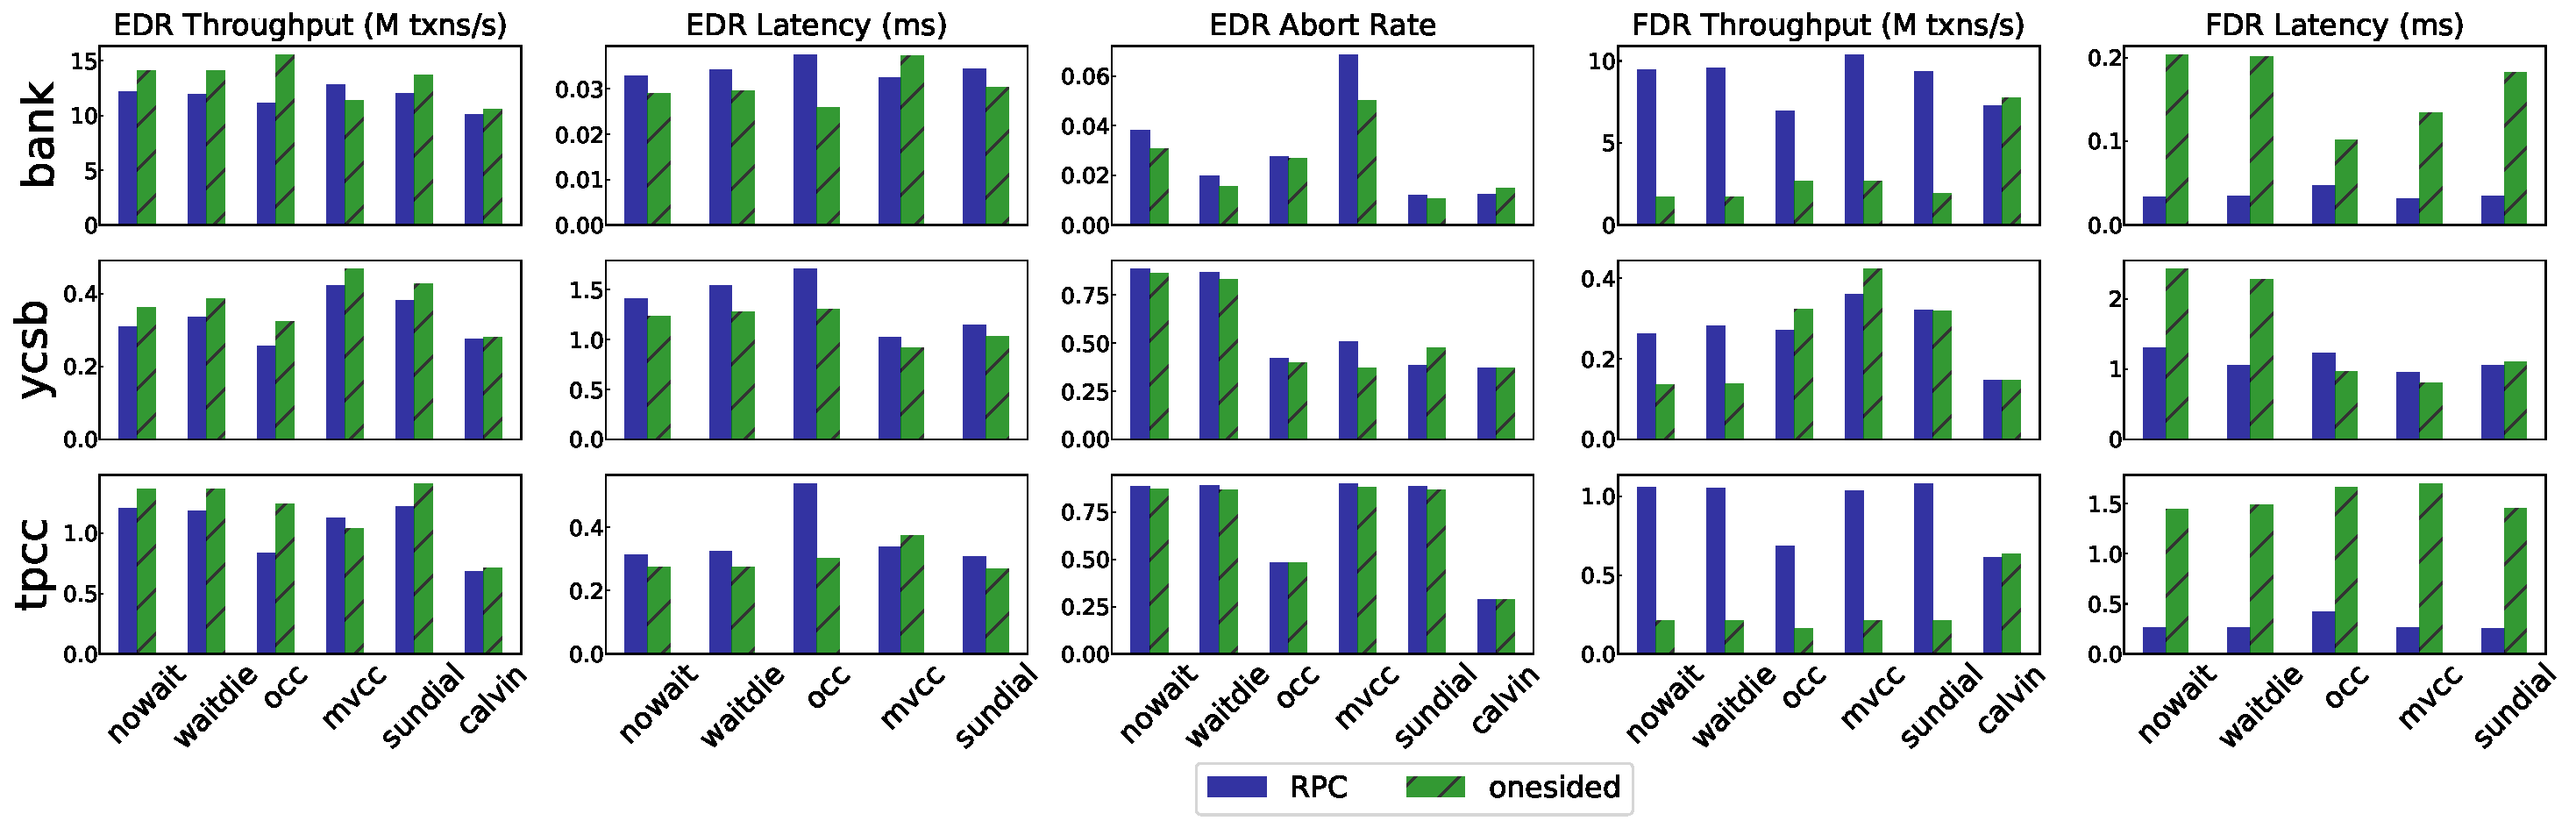
\includegraphics[width=18cm]{images/eval_overall.pdf}
    \vspace{-0.4cm}
    \caption{Overall throughput, latency for both EDR and FDR clusters and abort rates for the EDR cluster for all six protocols}
    \vspace{-0.7cm}
    \label{fig:eval_overall}
\end{figure*}

%\vspace{-2mm}
\subsection{Workloads}
%\vspace{-2mm}

We use three popular OLTP benchmarks, SmallBank~\cite{SmallBank}, YCSB~\cite{cooper2010benchmarking}, and TPC-C~\cite{TPC-C}, to test the performance of each protocol using two-sided RPC (denoted as \textbf{rpc}) or one-sided primitives (denoted as \textbf{onesided}). Records are partitioned across nodes. %To avoid effecting the results due to the assumption of locality, 
To eliminate the effects of locality, 
all transactions 
use network operations to fetch and update the data. 

\textbf{SmallBank}~\cite{SmallBank} is a simple banking application. Each transaction performs simple reads and writes on the account data. The key feature of SmallBank is that it has a small number of writes and reads in one transaction (in total less than four) with 
simple arithmetic operations.
%And its execution stage is quite simple. which is usually just one arithmetic operation. 
This makes SmallBank a network-intensive application. %Moreover, each record in SmallBank is of 4 bytes: it just stores simple information like checking and saving. It has six types of transactions, each sharing the same possibility of execution in our evaluations.

\textbf{YCSB}~\cite{cooper2010benchmarking} (The Yahoo! Cloud Serving Benchmark) is designed to evaluate large-scale Internet applications. There is just one table in the database. YCSB parameters such as
record size, the number of writes or reads involved in a transaction, the ratio of read/write and the skews are all configurable. In all our experiments, the record length is set to 64 bytes, with 1200000 entries in the table. We used hot area in YCSB, which consists of 1200 entries, i.e., 0.1\% of total records, to control contention. The number of table entries and hot area we use are proportional to the number of threads in \projectname. There are 10 operations in one transaction, with different read/write ratios.% in different experiments.
% In our test, an execution phase consuming 25\% of the whole transaction time is added to simulate the actual computation of a transaction.

\textbf{TPC-C}~\cite{TPC-C} simulates the processing of warehouse orders. In our evaluation, we run the transaction ``New-Order'', which consists of longer (up to 15) write sets and more complex transaction executions. In this benchmark, TPC-C has higher 
CPU utilization than SmallBank.

\vspace{-2mm}
\subsection{Execution Setup}
\vspace{-2mm}

We test our framework on two clusters, the first is an RDMA-capable cluster with 8 nodes. Each node is equipped with two 12-core Intel Xeon E5-2670 v3 processor, 128GB RAM and one ConnectX-4 EDR 100Gb/s InfiniBand MT27700. The second cluster is an RDMA-capable cluster with 16 nodes. Each node has two 8-core Intel Xeon CPU E5-2630 v3 processors, 64GB RAM, and one ConnectX-3 Pro FDR 56Gb/s InfiniBand MT27520. As there is only one RNIC on each node, we only run evaluations on the CPU on the same NUMA node with the RNIC to prevent NUMA from affecting our results. We name the first cluster EDR and the second cluster FDR in our experiments. We evaluate both \textbf{RPC} and \textbf{onesided} implementations of all \projectname protocols and focus on three metrics: {\em throughput, latency and abort rate}. To focus on comparing communication styles and protocols, we enforce coordinators to self-generate transaction requests.

\vspace{-2mm}
\subsection{Overall Results}
\vspace{-2mm}

% For six protocols, there are mainly three indicators to value the performance of the transaction protocol. They are throughput, latency and abort rate. These values are not independent, there are actually very complicated relationship between them.

Figure~\ref{fig:eval_overall} shows the overall results. In overall evaluations of YCSB, we have 20\% write and 80\% read and set the computation in the execution phase of YCSB to 5\% of the total latency of a transaction to simulate real-world applications. For evaluating throughput and abort rate, on the EDR cluster, we use 10 threads on each node and 10 co-routines for each thread, each co-routine producing and handling transaction requests independently. For the FDR cluster, we use 8 threads due to the limited number of cores in one CPU. %\blue{We use the }

%\begin{tcolorbox}
\underline{\bf Finding 1}: \textbf{Onesided} has a comparable or better throughput than \textbf{RPC} with only two exceptions for \mvcc on the EDR cluster (100Gb/s). 
%\end{tcolorbox}

\setlength{\intextsep}{2pt}%
\setlength{\columnsep}{8pt}%
\begin{wrapfigure}[5]{r}{.50\linewidth}
    \centering
    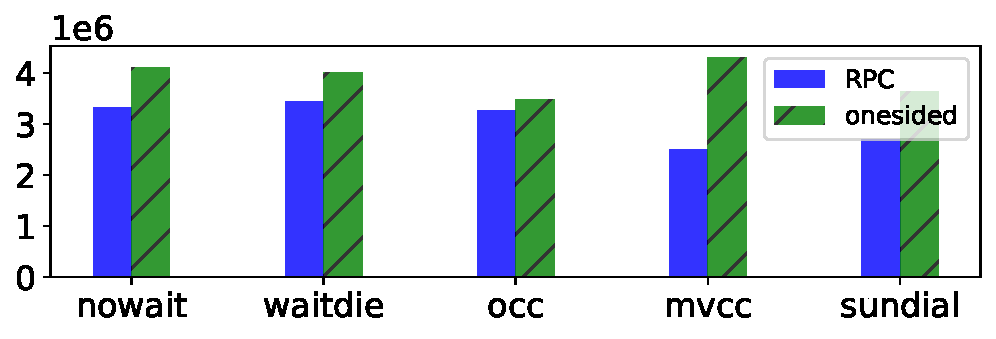
\includegraphics[width=\linewidth]{RCC-ISCA2020/images/network_trips.pdf}
    \vspace{-0.6cm}
    \caption{Network Round Trips}
    \vspace{-0.3cm}
    \label{fig:round-trips}
\end{wrapfigure}
We attribute \textit{Finding 1} to the fact that \textbf{onesided} can bypass remote CPUs, thus having a smaller communication overhead in general compared to their \textbf{RPC} counterparts for each round trip. This observation is true only when \textbf{onesided} implementations do not incur excessive amount of communication round trips compared to their \textbf{RPC} counterparts. However, this is not true for \mvcc. As we can see in Figure~\ref{fig:round-trips}, \textbf{onesided} \mvcc implementations incur 72\% more communication round trips while other protocols incur only a range of 6\% to 34\% more communication round trips. Therefore \textbf{RPC} is better than \textbf{onesided} for \mvcc on SmallBank and TPC-C. As for \mvcc on YCSB, which is a computation-intensive workload, \textbf{onesided} still dominates \textbf{RPC} even with 72\% more round trips; the advantage of bypassing remote CPUs becomes salient when remote CPUs are kept busy with computations.



%Such advantage of \textbf{onesided} becomes salient on computation-intensive workloads 
%\begin{tcolorbox}
\underline{\bf Finding 2}: While \textbf{onesided} is generally better than \textbf{RPC} on the EDR cluster (100Gb/s), \textbf{onesided} \occ is not necessarily the best protocol choice.
%\end{tcolorbox}

Protocols can be compared easily in \projectname. For SmallBank, which is a network-intensive benchmark and of low contention, \textbf{onesided} \occ is the best choice 
because it has the least number of network operations due to its optimistic assumption. For YCSB, which has more computation in the execution stage and more operations within one transaction, \textbf{onesided} \mvcc is the best. Moreover, it resolves many read-write conflicts by maintaining multiple versions of the records. So it has the lowest abort rate and highest throughput. For TPC-C, \textbf{onesided} \sundial is the best since it has the dynamic read lease and transaction timestamp. 

%\begin{tcolorbox}
\underline{\bf  Finding 3}: 
One-sided operations are not quite beneficial with 
low bandwidth (56Gb/s FDR). Only two protocols benefit from one-sided primitives under a computation-intensive workload.
%\end{tcolorbox}

%On the FDR cluster, one-sided operations are not well supported by the RNIC. 
On the FDR cluster, for read, write and lock requests, the latency of one-sided operations is 2.3x more than RPC with two-sided operations. The throughput and latency results of SmallBank shows that \textbf{RPC} is much better than \textbf{onesided} when the application is network bounded. YCSB, while having additional computation in the execution stage to increase co-routine execution time and burden remote CPUs, can still take advantage of the feature of \textbf{onesided} to bypass remote CPU and to outperform \textbf{RPC} for some protocols like \mvcc and \occ when the application is CPU-bounded. We do all experiments on the EDR cluster for later subsections.

On both clusters, the latency results essentially reflect similar conclusions as we have drawn from throughput results. As we use multiple (i.e., ten) co-routines to improve throughput, the latency of executing one transaction is adversely affected due to context switching. We will investigate latency breakdown by using just one co-routine later.

\vspace{-2mm}
\subsection{Impact of Co-routines}
\vspace{-2mm}

\begin{figure}[h]
    \centering
    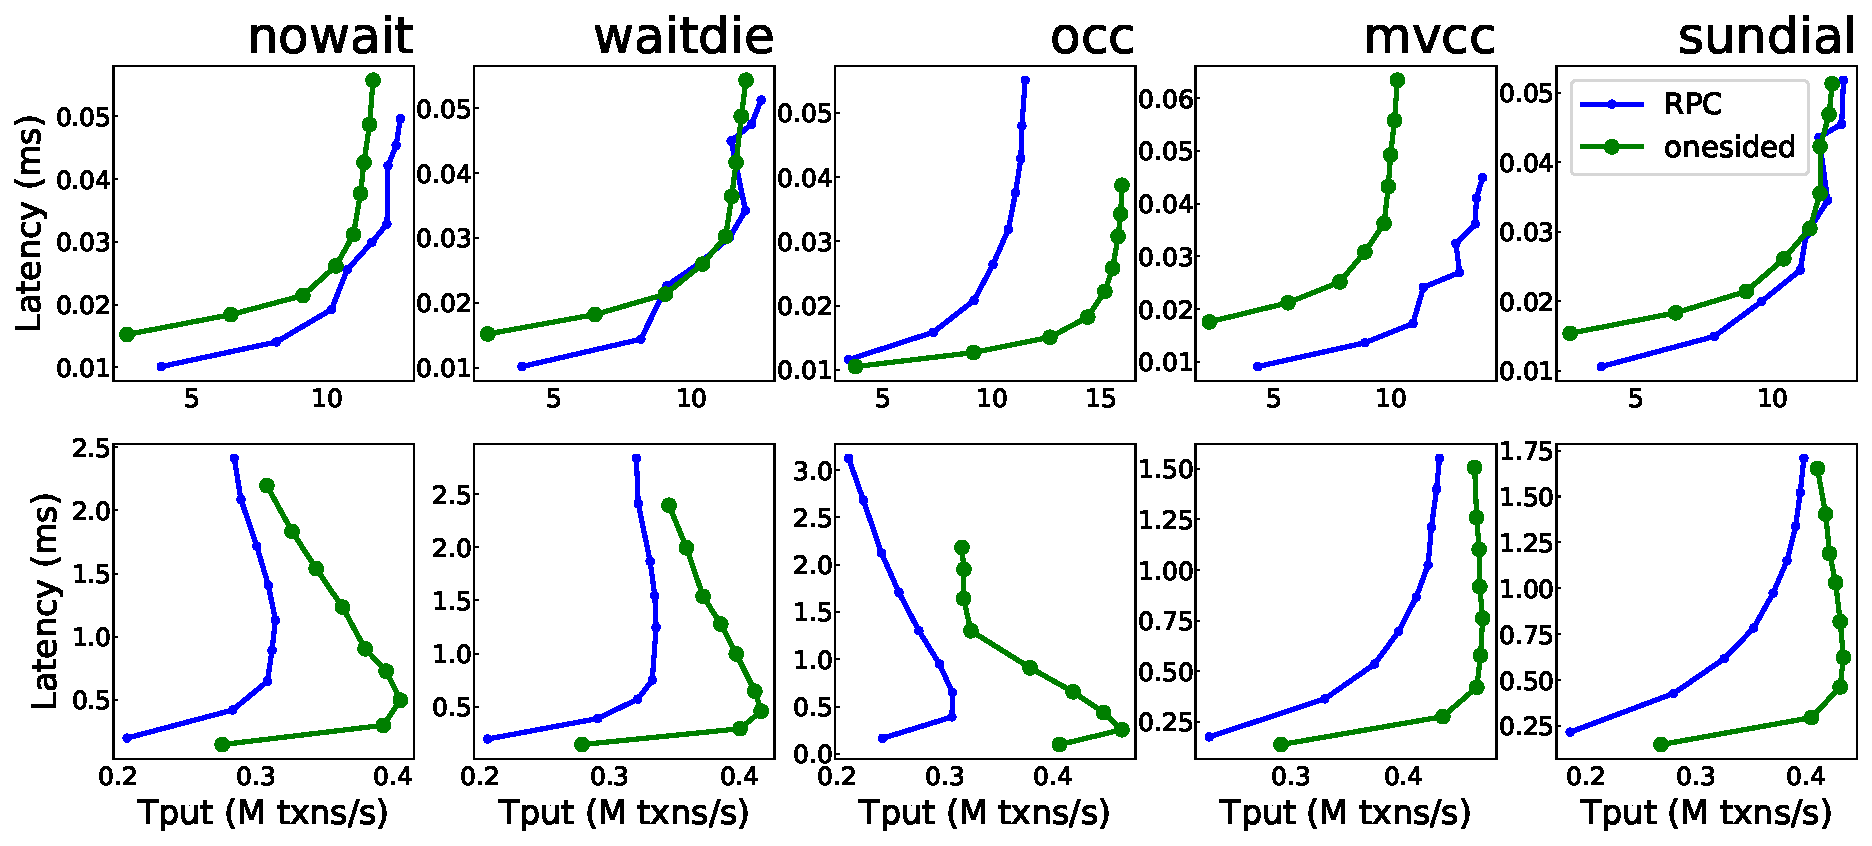
\includegraphics[width=8.5cm]{RCC-ISCA2020/images/latency-tput.pdf}
    \vspace{-0.4cm}
    \caption{Throughput and Latency for \textbf{SmallBank} (Up) and \textbf{YCSB} (Down) with co-routines ranging from 1 to 17 and a step of 2.}
    % \vspace{-0.2cm}
    \label{fig:coroutine-latency-tput}
\end{figure}

\begin{figure}[b]
    \centering
    \vspace{-0.6cm}
    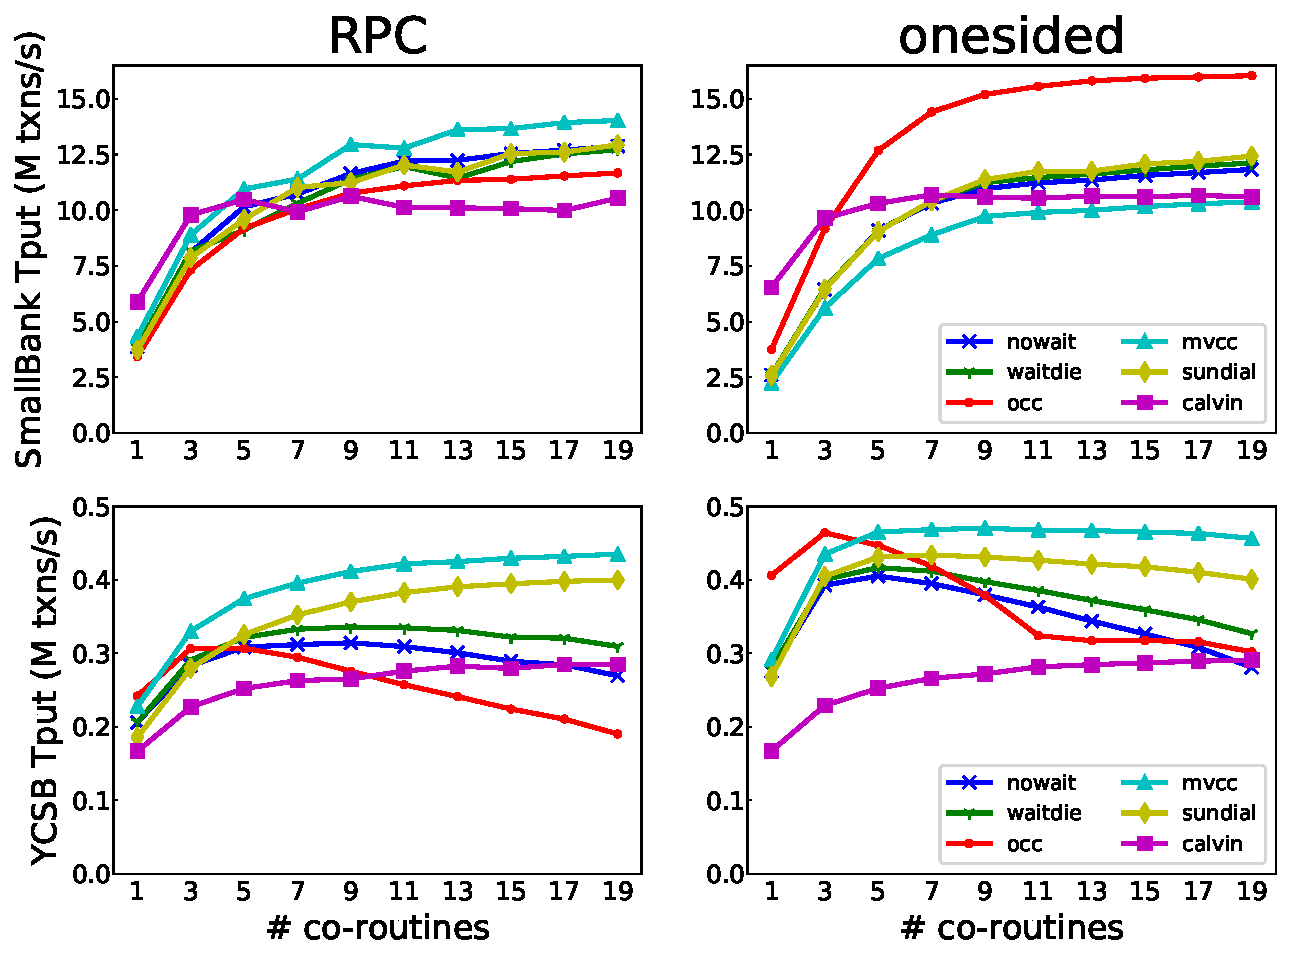
\includegraphics[width=0.8\linewidth]{images/eval_coroutines.pdf}
    \vspace{-0.4cm}
    \caption{The impact of \#co-routine to throughput}
    \vspace{-0.2cm}
    \label{fig:eval_cor_curve}
\end{figure}

To understand how co-routines affect the performance, we increase the co-routines from 1 to 17/19 with a step of 2 to test the latency and throughput in both SmallBank and YCSB. Results are reported on the EDR cluster. 

%\begin{tcolorbox}
\underline{\bf Finding 4}: The number of co-routines has great impact on the throughput and latency of both \textbf{RPC} and \textbf{one-sided} protocols while the best number of co-routines vary for different protocol implementations and different workloads. \projectname can provide a clear conclusion in making this design decision when building new transaction systems.
%\end{tcolorbox}

As seen in Figure~\ref{fig:coroutine-latency-tput}, on one hand, increasing the number of co-routines can help hide the latency of network operations, thus may improve throughput to some point. On the other hand, it will largely increase the latency of each transaction, leading to higher contention. This is because the tuples are locked for a longer time (2PL) or more likely to be interrupted for its longer life span (OCC). These two factors have different effects on SmallBank and YCSB.

As seen in Figure~\ref{fig:eval_cor_curve}, for SmallBank, the throughput of both \textbf{RPC} and \textbf{onesided} grow with the number of co-routines. As SmallBank is a network-intensive application, co-routines can greatly improve the throughput by overlapping the waiting time of network operations with transaction execution. As SmallBank touches few tuples in one transaction, there are even fewer tuples locked at the same time for \nowait and \waitdie, and the transaction has a shorter life span for \occ. Overall, the overlapping serves as the principal reason why throughput grows as \projectname uses an increasing number of co-routines. \textbf{Onesided} \occ has the most rapid growth in throughput because it locks records only at commit time, thus incurring the least conflict as co-routines increase. For \textbf{onesided} \mvcc and \sundial, which use more network operations for lower abort rate, the throughput is lower than that of the trivial protocols efficiently implemented in \textbf{onesided}.


For YCSB, which has more operations (i.e., 10) compared to SmallBank, more tuples are locked at the same time. Meanwhile, each transaction takes more time to finish, making records be locked even longer. Under this scenario, using more co-routines may significantly increase contention and adversely affect throughput after a critical point for some protocols, as seen in Figure~\ref{fig:coroutine-latency-tput} and Figure~\ref{fig:eval_cor_curve}. Among \textbf{RPC} implementations of all protocols, for those that can better handle read-write conflicts, i.e., \mvcc and \sundial, their throughput can continue growing as the number of co-routines increases. Recall that \mvcc keeps old versions for read operations and that \sundial dynamically chooses the transaction timestamp and updates the read lease. But protocols like \nowait and \waitdie, which lock all tuples involved in read and write operations, suffer from longer locked tuples with more co-routines. \occ 
is designed for the low contention scenario. 
%is aimed at performing efficiently when there is not much conflict. 
As we mentioned before, with more computation in the execution stage \occ has higher abort cost. So increasing the number of co-routines exacerbates its performance. \calvin performance is mainly bounded by the computation, because each coordinator that actively participates in a transaction has to perform the time-consuming execution stage even the transaction was not initiated by its own sequencing stage, leading to lower effective throughput. 

Comparing the execution of \nowait, \waitdie and \occ implementations on SmallBank and YCSB, we observe that the optimal co-routine number gets smaller as a transaction touches more records. \projectname can draw useful conclusions as such for future RDMA-based transaction system builders when they consider optimizing system throughput.

\vspace{-2mm}
\subsection{Impact of Contention Level}
 \vspace{-2mm}



To show how well RDMA-based protocols can handle contention, we compare the throughput of six protocols with different contention levels for YCSB. We control the contention levels by varying the possibility of one read or write visiting a small portion of data records, i.e., hot area. 
% Another parameter is the read/write ratio for one transaction. In our experiments, the read/write ratio is 1:4.
% Moreover, we also simulate execution stage by doing dummy computation which takes 5\% of the total latency of a full transaction.
The results (on EDR cluster) are shown in Figure~\ref{fig:eval_conflict_level}. 


\begin{figure}[htp]
    \centering
    \vspace{-0.2cm}
    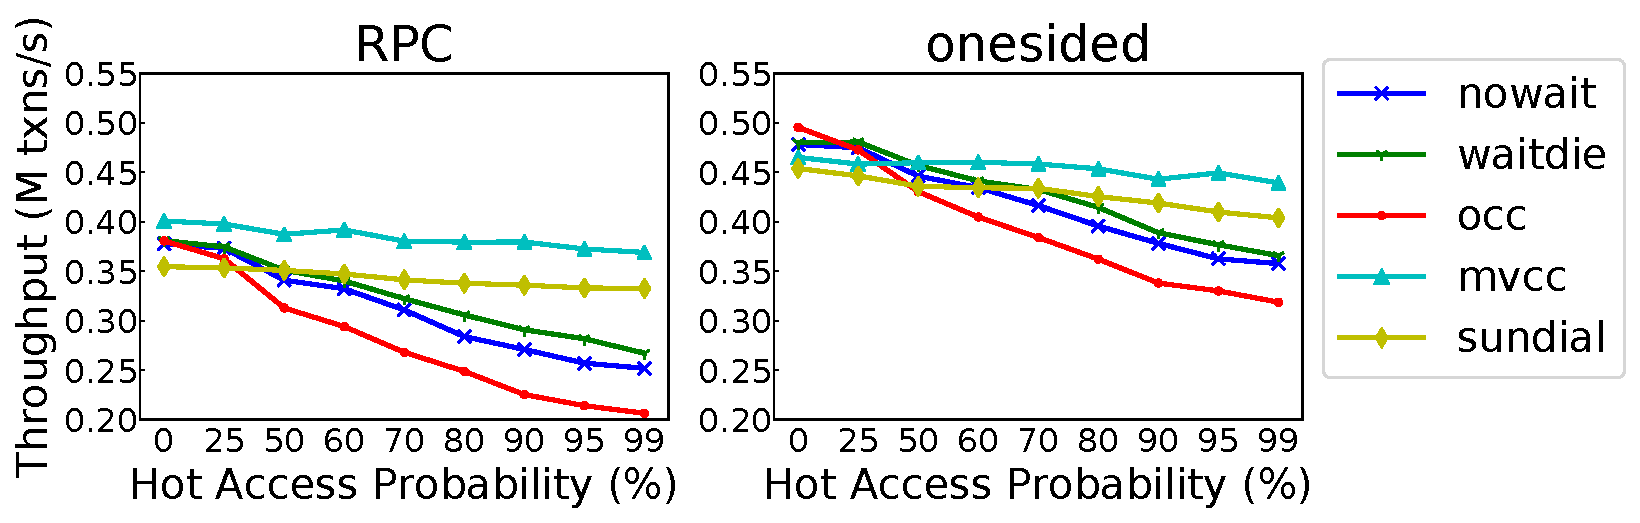
\includegraphics[width=0.8\linewidth]{images/eval_conflict.pdf}
    \vspace{-0.4cm}
    \caption{The impact of contention level to throughput for YCSB}
    \vspace{-0.8cm}
    \label{fig:eval_conflict_level}
\end{figure}

%\begin{tcolorbox}
\underline{\bf Finding 5}: The throughput of different protocol implementations drop at different rates for both \textbf{RPC} and \textbf{onesided}. \mvcc \textit{always} outperforms the state-of-the-art \sundial irrespective of contention levels.
%\end{tcolorbox}

In both \textbf{RPC} and \textbf{onesided} implementations, performance of \occ decreases most sharply because of larger possibility to abort and high abort cost due to its optimistic assumption under a high contention level. The performance of \nowait and \waitdie significantly decrease due to the intensive conflict read and write locks. \mvcc and \sundial are less affected when the conflict rate increases; their throughput decrease is slow because they have optimization to avoid read-write conflict. \calvin is not affected much by different contention levels because a \calvin transaction only locks local records for a short period without necessarily waiting for remote locks. This behavior of \calvin is confirmed in~\cite{Thomson:2012:CFD:2213836.2213838}.

%The effect brought by conflict rate similarly effect the \textbf{onesided} and \textbf{rpc} version, because the performance difference mainly come from the algorithm here.
We also notice that \textbf{onesided} \sundial and \mvcc, although featuring good read-write conflict management, are worse than \textbf{onesided} \occ when a transaction has the least conflict rate. That is because these two have more complicated operations to maintain more information to reduce the abort rate, which is more costly because every access to remote data will trigger network operation in \textbf{onesided} version.

%\blue{TODO: \calvin and contention}

It is worthwhile to note that \mvcc is consistently better than \sundial irrespective of contention levels in both \textbf{RPC} and \textbf{onesided} implementations for YCSB. While we do not expect \cite{yu2018sundial} to compare with all previous concurrency control protocols under all possible workloads, our \projectname's results show a strong indication that \sundial is worse than one variant of \mvcc implementations when the workload is computation-intensive in the RDMA context. This non-trivial observation would not possible without our unified RDMA-based concurrency control framework. 

\vspace{-2mm}
\subsection{Impact of Execution Workloads}
%\vspace{-2mm}

\begin{figure}[htp]
    \centering
    \vspace{-0.2cm}
    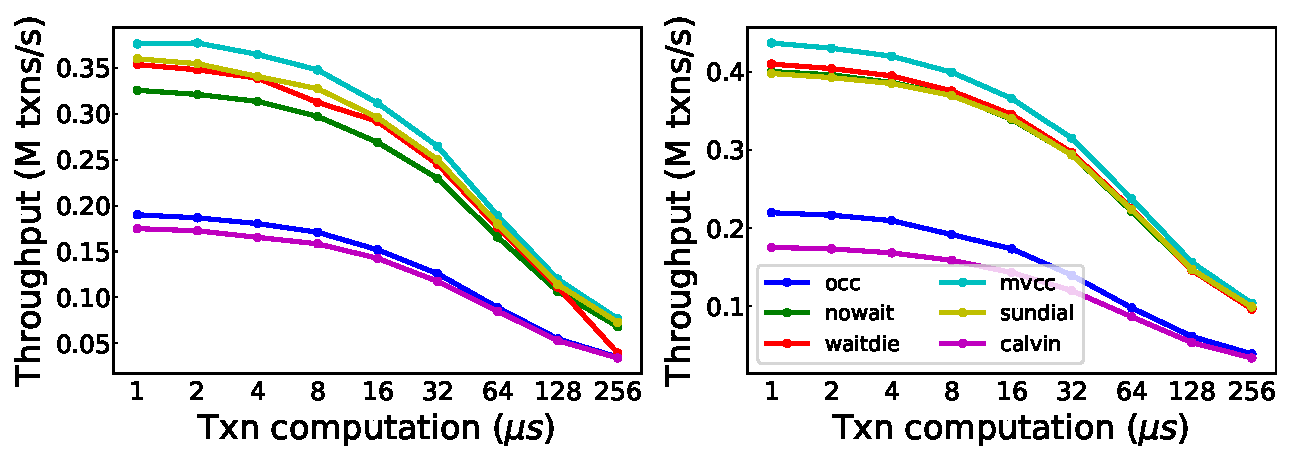
\includegraphics[width=0.8\linewidth]{images/eval_exe_workload.pdf}
    \vspace{-0.4cm}
    \caption{The impact of computation workload to throughput}
    \vspace{-0.2cm}
    \label{fig:eval_sleep_curve}
\end{figure}

% As shown in the overall results, \textbf{onesided} version can better handle transactions bounded by computation. 
%So we increase the percentage of the computation in one transaction. 
To study the implication of computation ratio, we add dummy computation in the execution stage of YCSB, ranging from 1 to 256 $\mu$s. We carry out experiments on the EDR cluster and show results in Figure~\ref{fig:eval_sleep_curve}.

%\begin{tcolorbox}
\underline{\bf Finding 6}: \textbf{RPC} and \textbf{onesided} share similar decreasing trend with increasing computation workload at execution stage; \textbf{onesided} always outperforms \textbf{RPC} for different computation workloads.
%\end{tcolorbox}

%We can see the same trend that the throughput decrease with increasing computation at execution stage for . Yet \textbf{onesided} version always outperforms \textbf{rpc} version under different computation workloads. 

%Moreover, \textbf{onesided} version have a slower decreasing trend. 

In \textbf{RPC} versions, more computation time on the execution stage causes higher latency for an RPC request to get handled, which significantly increases the time that a tuple is locked, leading to higher abort rate. \textbf{onesided} versions are also adversely affected yet have a relatively slower decreasing trend. 
Suffering from both high abort cost and long computation time, \occ performs much worse than 2PL protocols. \calvin's performance is bounded by local computation; thus, there is no difference between {\bf RPC} and \textbf{onesided} version.






% -- For the following sections, please check OSDI and VLDB papers carefully and try to include all results we can get similar to them. We can organize sections later. 

% -- We can first include all experiments summarized by Kezhao, and go over again **each** result figure of the two papers, and ask whether we can get it and whether it is needed (or how can several be combined into one)? We want to provide a superset of results
% compared to the two. We should pay special attention to the findings **unknown** before or **unexpected**.

% -- We will not have a "discussion" section after the Evaluation, instead you need to analyze the results in detail in each subsection here. 

% \begin{figure}[htp]
%     \centering
%     \includegraphics[width=6cm]{images/overall_throughput_10thread_10_cor.pdf}
%     \caption{Overall Throughput}
%     \label{fig:overall_tput}
% \end{figure}

% \begin{figure}[htp]
%     \centering
%     \includegraphics[width=6cm]{images/overall_abort_10thread_10_cor.pdf}
%     \caption{Overall Abort Rate}
%     \label{fig:overall_abort}
% \end{figure}


% \begin{figure}
%   \centering
%   \begin{tabular}{@{}c@{}}
%     \includegraphics[width=.8\linewidth,height=50pt]{images/latency_of_operations_small_bank_10_thread_1_cor.pdf} \\[\abovecaptionskip]
%     \small (a) 10 threads 1 co-routine
%   \end{tabular}

%   \vspace{\floatsep}

%   \begin{tabular}{@{}c@{}}
%     \includegraphics[width=.8\linewidth,height=50pt]{images/latency_of_operations_small_bank_10_thread_5_cor.pdf} \\[\abovecaptionskip]
%     \small (b) 10 threads 5 co-routines
%   \end{tabular}
  
%   \begin{tabular}{@{}c@{}}
%     \includegraphics[width=.8\linewidth,height=50pt]{images/latency_of_operations_small_bank_10_thread_10_cor.pdf} \\[\abovecaptionskip]
%     \small (b) 10 threads 10 co-routines
%   \end{tabular}
  
%   \begin{tabular}{@{}c@{}}
%     \includegraphics[width=.8\linewidth,height=50pt]{images/latency_of_operations_small_bank_10_thread_15_cor.pdf} \\[\abovecaptionskip]
%     \small (b) 10 threads 15 co-routines
%   \end{tabular}

%   \caption{Latency break down in small bank}\label{fig:lat_break_down}
% \end{figure}

% \begin{figure}
%   \centering
%   \begin{tabular}{@{}c@{}}
%     \includegraphics[width=.8\linewidth,height=50pt]{images/latencyycsb_cor1.pdf} \\[\abovecaptionskip]
%     \small (a) 10 threads 1 co-routine
%   \end{tabular}

%   \vspace{\floatsep}

%   \begin{tabular}{@{}c@{}}
%     \includegraphics[width=.8\linewidth,height=50pt]{images/latencyycsb_cor5.pdf} \\[\abovecaptionskip]
%     \small (b) 10 threads 5 co-routines
%   \end{tabular}
  
%   \begin{tabular}{@{}c@{}}
%     \includegraphics[width=.8\linewidth,height=50pt]{images/latencyycsb_cor10.pdf} \\[\abovecaptionskip]
%     \small (b) 10 threads 10 co-routines
%   \end{tabular}
  
%   \begin{tabular}{@{}c@{}}
%     \includegraphics[width=.8\linewidth,height=50pt]{images/latencyycsb_cor15.pdf} \\[\abovecaptionskip]
%     \small (b) 10 threads 15 co-routines
%   \end{tabular}

%   \caption{Latency break down in YCSB}\label{fig:lat_break_down}
% \end{figure}


% \begin{figure}
%   \centering
%   \begin{tabular}{@{}c@{}}
%     \includegraphics[width=.9\linewidth,height=50pt]{images/latency_of_operations_small_bank_10_thread_1_cor.pdf} \\[\abovecaptionskip]
%     \small (a) 10 threads 1 co-routine smallbank
%   \end{tabular}

%   \vspace{\floatsep}

%   \begin{tabular}{@{}c@{}}
%     \includegraphics[width=.9\linewidth,height=50pt]{images/latencyycsb_cor1.pdf} \\[\abovecaptionskip]
%     \small (b) 10 threads 1 co-routines YCSB
%   \end{tabular}
%   \caption{Latency break down}\label{fig:lat_break_down}
% \end{figure}

% We tested the break down time cost in each stage of five protocols with co-routine number ranging from 1 to 15 in small bank and YCSB. We can see that RPC and \textbf{onesided} version have very different performance between small bank and YCSB. In small bank, with different co-routine number, RPC always outperforms \textbf{onesided} in read and lock\&read. This is because in out RPC implementation, a read can be done by launching just one RPC request. No matter if the stage needs complex operations(for example in MVCC, it should traverse all the time stamps and find the suitable one to read), RPC handler can locally access the data and check the time stamps. However, for \textbf{onesided}, any data access will be remote so as to be costly. Especially when \textbf{onesided} has to check the correctness of data, it should re-read the write time stamp after reading the real data, to guarantee the atomicity of reading. In this case, two RDMA read requests will be launched. For lock\&read operation, for protocols using waitdie deadlock prevention method, once a lock fails and the one with high priority would retry. For \textbf{onesided}, one retry means one RDMA atomic operation. But for RPC, the retry can be done locally within the handler. High contention will lead to more RDMA atomic requests for retry, causing heavier network traffic. The side effect also show on the throughput results. As a result in small bank and TPCC, the RPC of different protocols all outperform \textbf{onesided} with similar abort rate. 

% However, in YCSB with execution phase, we have the different results. Latency of RPC is at least three times higher than \textbf{onesided} version. We add some dummy execution workload into YCSB which takes 25\% of the whole transaction time to simulate excution in real-world transaction. And in this time, the CPU will be busy and become the bottleneck of the process. In the RPC version, the RPC requests should be handled by the remote node. As the remote node is busy doing the tasks in the execution phase, in average it will take much longer time for the handler to handle the RPC request. But for \textbf{onesided} version, as the one-sided operations bypass the remote CPU, the latency remains the same with the transactions in the benchmarks that are with low CPU utilization. In this condition, \textbf{onesided} outperforms RPC in both latency and throughput.

\vspace{-2mm}
\subsection{System Resource Utilization}
%\vspace{-2mm}

%\begin{tcolorbox}
\underline{\bf Finding 7}: \textbf{Onesided} implementations are less likely to be bottlenecked by system resources and can reach much higher network utilization than their \textbf{RPC} counterparts.
%\end{tcolorbox}

We measure system resource utilization of both \textbf{RPC} and \textbf{onesided} implementations by two experiments. First, we use two different thread numbers (i.e., five threads and ten threads) of all implementations on the EDR cluster for the YCSB benchmark and show the throughput increase in Table~\ref{tbl:two-threads}. Since our \projectname is symmetric: i.e., each co-routine in some thread only communicates with another co-routine at the {\em same thread} of another machine. Ideally, doubling thread numbers would also doubling the throughput increase if not bottlenecked by system resources and if we did not consider the effect of an increased contention level. In reality, from Table~\ref{tbl:two-threads}, we can see that \textbf{onesided} implementations are equally or more closer to the ideal case, thus having equal or less likelihood of being bottlenecked by system resources as \textbf{RPC} implementations. This behavior is understandable since \textbf{onesided} implementations bypass system calls and kernels, thus avoiding many possibilities of being bottlenecked. \textbf{Onesided} \sundial is the protocol that is closest to linear scalability in \projectname. Overall, \projectname provides researchers with the opportunity to compare RDMA-based protocols in terms of system utilization. We leave pinpointing the exact system resource bottleneck for each protocol as an important future work.

Second, to characterize the network utilization of different protocols in both \textbf{RPC} and \textbf{onesided} implementations, we measure their message rates in \projectname when executing for the YCSB workload on the EDR cluster. Table~\ref{tbl:message-rate} shows our results. We observe the max message rate in RCC reaches 31.06 Mpps by \textbf{onesided} \nowait. Given that the RDMA peak message rate of our {EDR} cluster is 33 Mpps, \textbf{onesided} \nowait has reached 94.1\% of the peak. On average \textbf{onesided} implementations send approximate {\em twice} more packages per second than their \textbf{RPC} counterparts, which indicates that \textbf{onesided} protocols all have much higher network utilization. 




% We believe in a cluster with lower network performance, RCC can show different bottlenecks.



\subsection{Stage Latency Breakdown}

While we have already done some experiments to compare various aspects of different protocols in \projectname. Previous latency results are still not an accurate reflection of the actual bottleneck of each protocol since interleaving transactions among multiple co-routines increases transaction latency nondeterministically. In order to pinpoint the stage-wise bottleneck of each protocol implementation further, we run all implementations except \calvin using {\em only one} co-routine for SmallBank on 4 nodes of {EDR} cluster and break down a whole transaction latency into different stages: \textit{Read}, \textit{Lock}, \textit{Release}, \textit{Commit}. \sundial has an extra lease \textit{Renew} latency. \calvin is not included in this experiment because all these stages are local operations for \calvin. Figure~\ref{fig:latency-breakdown} shows the stage-wise latency breakdown. Note that for \textbf{RPC} \nowait and \waitdie, a record is returned together with locking result (as a  whole tuple), so their \textit{Read} latency is combined into the \textit{Lock} latency.

\begin{table}[h!]
\vspace{-2mm}
\caption{Thoughput in K/s for different threads on EDR}
\vspace{-2mm}
\centering
\begin{tabular}{|c|c|c|c|c|c|c|}
 \hline
  &
 \multicolumn{3}{|c|}{\textbf{RPC}} &
 \multicolumn{3}{|c|}{\textbf{onesided}} \\
 \hline
 \#threads & 5 & 10 & & 5 & 10 & \\
 \hline
 nowait & 40.23	& 67.9 & 1.69x &	56.83 & 107.44 & 1.89x \\
 \hline
 waitdie & 40.12 & 71.69 & 1.79x & 57.26 & 102.08 & 1.78x \\
 \hline
 occ & 27.45 & 48.09 & 1.75x & 47.93 & 84.53 & 1.76x \\
 \hline
 mvcc & 52.34 & 91.93 & 1.76x & 68.16 & 125.61 & 1.84x \\
 \hline
 sundial & 50.28 & 80.68 & 1.60x & 60.26 & 119.19 & 1.98x \\
 \hline
\end{tabular}
\label{tbl:two-threads}
\end{table}


\begin{table}[h!]
\vspace{-0mm}
\caption{Msg. Rate in M pkgs/s on EDR and utilization}
\vspace{-3mm}
\centering
\begin{tabular}{|c|c|c|c|}
 \hline
  &
 \textbf{RPC} & 
 \textbf{onesided} & network utilization \% \\
 \hline
 nowait & 9.49 & 31.06 & $28.8 \rightarrow 94.1$ \\
 \hline
 waitdie & 9.25	& 30.77 &  $28.0 \rightarrow 93.2$ \\
 \hline
 occ & 9.75 & 30.38 & $29.5 \rightarrow 92.1$   \\
 \hline
 mvcc & 10.70 & 28.46 & $32.4 \rightarrow 86.2$ \\
 \hline
 sundial & 9.91	& 29.52 & $30.0 \rightarrow 89.5$  \\
 \hline
\end{tabular}
\vspace{-0mm}
\label{tbl:message-rate}
\end{table}

For \textbf{RPC} implementations, as illustrated in Figure~\ref{fig:latency-breakdown}, \mvcc incurs the largest \textit{Read} latency due to the participant's traversal of the all \texttt{wts} of the requested record. \mvcc also incurs the largest \textit{Lock} latency due to the participant's double checking of conditions for successful locking. \occ incurs the largest latency at \textit{Commit} and \textit{Release} stages and second largest \textit{Read} latency compared to other protocols. This is because the \occ implementation of \cite{wei2018deconstructing} accumulates all RPC read/write messages in one stage into one message before broadcasting it to all participants, which uses higher network bandwidth and incurs larger latency (This latency is not apparent with ten co-routines as in Figure~\ref{fig:eval_overall}). 

For \textbf{onesided} implementations, as illustrated in Figure~\ref{fig:latency-breakdown}, \textit{Release} is not the bottleneck for any protocol. \mvcc and \sundial suffers from the top-2 \textit{Read} latency due to their extra logic for ensuring valid record version or valid lease upon read operations. \mvcc suffers from the largest \textit{Lock} latency since it needs to retrieve longer metadata upon locking using \texttt{CAS}. 
%\occ suffers from the largest \textit{Release} and \textit{Commit} latency since \red{xxx}.

By analyzing stage latency results, researchers can make use of \projectname to understand better and mitigate the stage-wise bottlenecks of \textbf{RPC} and \textbf{onesided} implementations.

\vspace{-2mm}
\subsection{Comparison with the State-of-the-art}
\vspace{-2mm}

As we have stated that \projectname is the {\em first} unified framework of RDMA-based implementations of representative protocols. There is no apple-to-apple comparison for each protocol. We implemented five TCP-based RPC versions in \projectname and compared these TCP protocols in \projectname with corresponding TCP-based protocols in \cite{harding2017evaluation} and \cite{yu2018sundial}  using similar configurations on YCSB. Table~\ref{tbl:compare-with-stoa} shows the results.
As we can see, except \sundial, our TCP implementations are comparable or better than corresponding implementations in \cite{harding2017evaluation}. The two-sided RDMA versions in \projectname perform an order of magnitude better than corresponding TCP versions in \projectname or \cite{harding2017evaluation}.



\begin{table}[h!]
\vspace{-2mm}
\caption{Comparing throughput (Txns/s) of \projectname with the State-of-the-Art protocol implementations using TCP. }
\vspace{-2mm}
\centering
\begin{tabular}{|c|c|c|c|}
 \hline
  &
 Other TCP-based 
  & 
 \projectname TCP-based
  &
 \projectname Two-sided  
 \\
 \hline
 nowait & approx. 50000~\cite{harding2017evaluation} & 48394 & 308177 \\
 \hline
 waitdie & approx. 10000~\cite{harding2017evaluation} & 51444 & 336514 \\
 \hline
 occ & approx. 40000~\cite{harding2017evaluation} & 49949 & 257307 \\
 \hline
 mvcc & approx. 20000~\cite{harding2017evaluation} & 63514 & 420000 \\
 \hline
 sundial & approx. 70000~\cite{yu2018sundial} & 38275 & 383237 \\
 \hline
 % calvin & ~120000~\cite{harding2017evaluation} & - & 281426 \\
%  \hline
\end{tabular}
\vspace{-0.4cm}
\label{tbl:compare-with-stoa}
\end{table}

\begin{figure}[h]
    \centering
    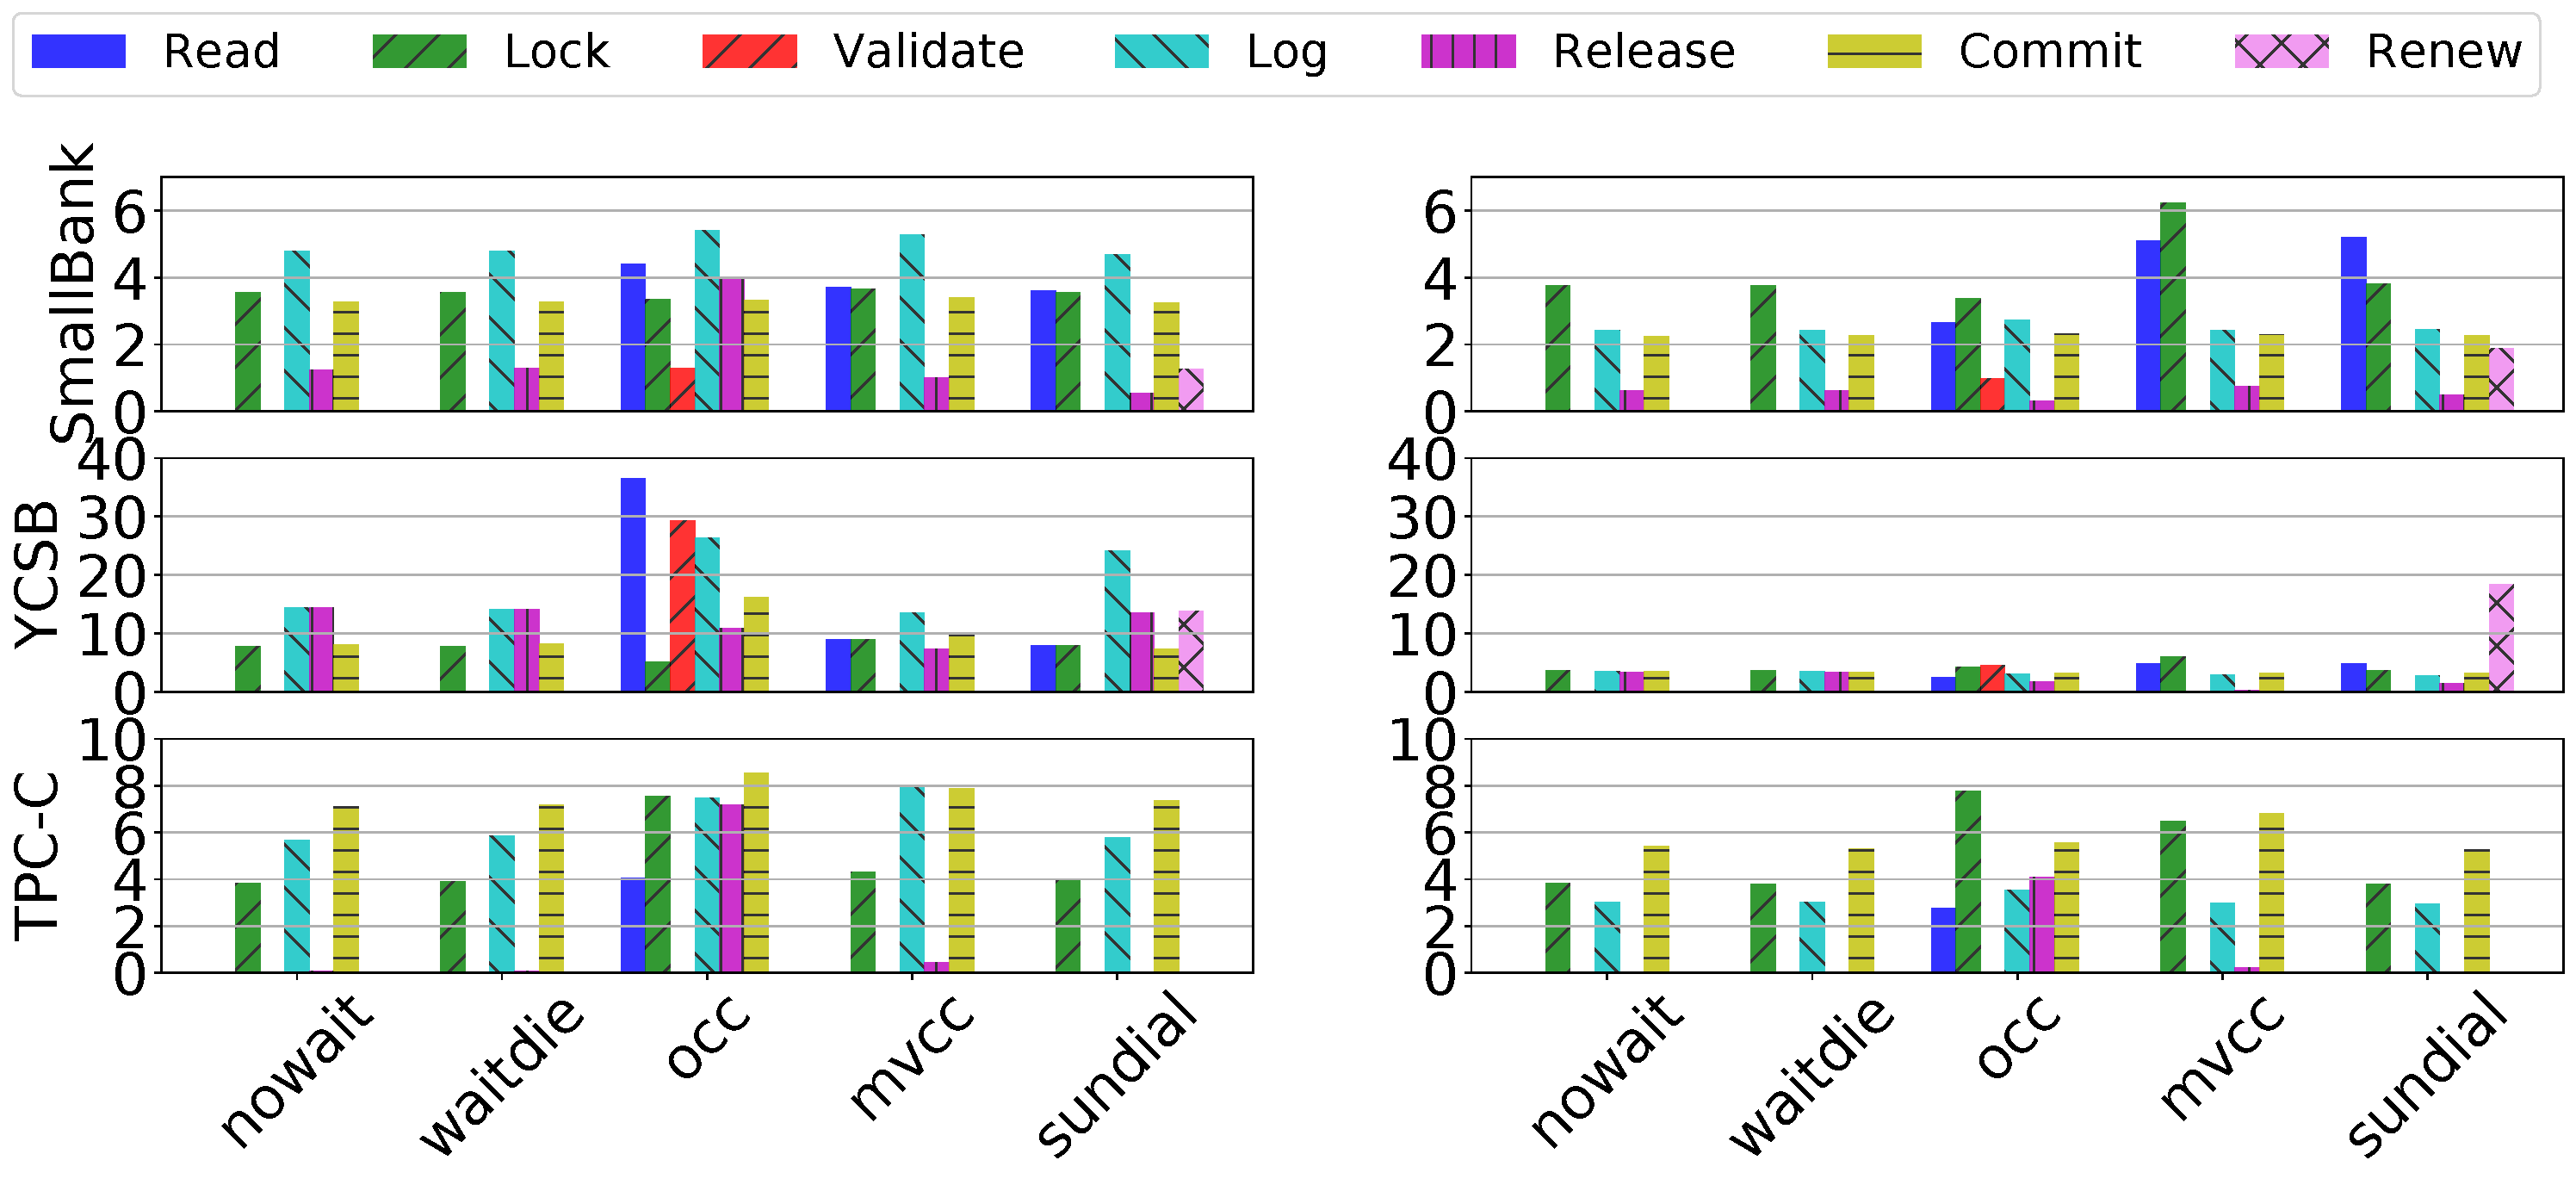
\includegraphics[width=0.8\linewidth]{RCC-ISCA2020/images/lat_breakdown.pdf}
    \vspace{-0.4cm}
    \caption{Latency breakdown for \textbf{RPC} (Left) and \textbf{onesided} (Right)}
    \vspace{-0.6cm}
    \label{fig:latency-breakdown}
\end{figure}


%\vspace{-2mm}
\section{Related Work}
%\vspace{-2mm}
{\bf Comparisons among concurrency control protocols}
%Prior work has made valuable comparisons on different concurrency control protocols. 
\cite{agrawal1987concurrency} uses modeling techniques to reveal the hidden connections between protocols' underlying assumptions and their seemingly contradictory performance results.\cite{huang1991experimental} compares three concurrency control protocols in real-time database systems but only restraints to optimistic ones. \cite{yu2015evaluation,yu2014staring} focuses on the scalability issues and examines seven concurrency control protocols on a main-memory DBMS on top of a simulated 1024-core system.  Deneva~\cite{harding2017evaluation} is the recent work comparing distributed concurrency control protocols in a single unified framework. 
%Deneva executes all transactions as stored procedures that run on servers, and analyzes the performance of different protocols under different settings like network speed, node number, update rate and contention. 
\projectname 
takes the first step in comparing different protocols under the context of various RDMA primitives.

{\bf Comparisons between RDMA primitives}
%Before \projectname, there has already been work comparing RDMA primitives. 
\cite{kaminsky2014using} compares the use of RDMA \texttt{WRITE} and RDMA \texttt{READ} when constructing a high performance key-value system. \cite{dragojevic2014farm} finds out that RDMA \texttt{WRITE}'s polling significantly outperforms \texttt{SEND} and \texttt{RECV} verbs when constructing the FaRM's communication subsystem. \cite{kalia2016fasst} shows that UD-based RPC using \texttt{SEND} and \texttt{RECV} outperforms one-sided primitives. \cite{wei2018deconstructing} did more primitive-level comparisons with different payload size. Compared
to them, \projectname compare the primitives
with a much wider range of concurrency control algorithms
on two clusters with different RDMA capabilities.

%applicRDMA nation level in order to reach useful insights in constructing concurrency control protocols.

{\bf Distributed transaction systems}
High performance transaction systems have been investigated intensively~\cite{Thomson:2012:CFD:2213836.2213838,corbett2013spanner,tu2013speedy,dragojevic2015no,chen2016fast,wei2018deconstructing,lee2015implementing}. Most of them focus on distributed transaction systems~\cite{corbett2013spanner,dragojevic2015no,chen2016fast,wei2018deconstructing} since it is more challenging to implement a high performance transaction system with data partitioned across the nodes. 
Some works, e.g., \cite{lee2015implementing,dragojevic2015no,chen2016fast,wei2018deconstructing,kalia2016fasst}, focus only on one protocol (i.e., some variants of \occ). Other works like~\cite{wei2015fast,yu2018sundial,Thomson:2012:CFD:2213836.2213838} explore novel techniques like determinism or leasing. However, these works did not explore the opportunity of using RDMA networks.

%\vspace{-2mm}
\section{Conclusion}
%\vspace{-2mm}

In this paper, we build {\em \projectname}, the first
unified RDMA-enabled distributed transaction processing framework supporting 
six concurrency control protocols 
using either two-sided or one-sided primitives.
We intensively optimize the performance
using techniques such as co-routines, outstanding requests, and
doorbell batching.
Based on \projectname, we conduct the first
and most comprehensive
(to the best of our knowledge) comparison
of different representative distributed
concurrency control protocols 
on two clusters with different 
RDMA network capabilities.

%%%%%%% -- PAPER CONTENT ENDS -- %%%%%%%%


%%%%%%%%% -- BIB STYLE AND FILE -- %%%%%%%%
\bibliographystyle{IEEEtranS}
\bibliography{references}
%%%%%%%%%%%%%%%%%%%%%%%%%%%%%%%%%%%%

\end{document}

